%% LyX 2.0.3 created this file.  For more info, see http://www.lyx.org/.
%% Do not edit unless you really know what you are doing.
\documentclass[english,mtech,noded,noack,nosyn]{desethesis}
\usepackage{mathptmx}
\usepackage{helvet}
\usepackage{courier}
\usepackage{float}
\usepackage{graphicx}
\usepackage{tabularx}
\usepackage{subcaption}
\usepackage{fixltx2e}
\usepackage{pdfpages}
\graphicspath{{images/}}
\renewcommand{\thetable}{\Roman{table}}
\renewcommand{\familydefault}{\rmdefault}
\usepackage[latin9]{inputenc}
\setcounter{secnumdepth}{3}
\setcounter{tocdepth}{3}

\makeatletter
%%%%%%%%%%%%%%%%%%%%%%%%%%%%%% User specified LaTeX commands.

%Options for type of thesis
% phd   - for PhD thesis at IISc
% mtech - for MTech dissertation at IISc
% me    - for ME dissertation at IISc

%Options to disallow following preliminary pages if you intend to include it as a file in the mainmatter
% noded  - dis-allows the Dedication page
% noack  - dis-allows the Acknowledgements page
% nosyn  - dis-allows the Synopsis page
%------------------------------------------------------------------------------------------
% Thesis details
  \Year{2016}
  \Month{June}
  \Author{Jayraj Desai\\\&\\Robin Singh Nanda}
  \Advisor{Prof. Bharadwaj Amrutur}
  \CoAdvisorB{}
  \Title{Connected Panic Button with audio-based trigger}
  \Dedication{}
  \Synopsis{}
  \Keywords{}
  \Acknowledgments{}
 %------------------------------------------------------------------------------------- 
 

\makeatother

\usepackage{babel}
\addto\captionsenglish{\renewcommand{\figurename}{Fig.}}
\begin{document}
\frontmatter \makepreliminarypages \singlespace


\chapter*{Synopsis}

In this report, we propose a safety-service that helps to reduce criminal offense count in public transport vehicles. A device called \emph{PanicButton device}* mounted in these vehicles is at the core of this service. The \emph{PanicButton device} is equipped with wireless modules like Global System for Mobile communications (GSM) for ubiquitous connectivity to the back-end servers and bluetooth low energy (BLE) for communicating with the users. To make the \emph{PanicButton device} user friendly, we restrict physical user interface to only a panic button. The \emph{PanicButton device} runs algorithm to detect any tampering and also provide smart-phone based validation. Audio-based trigger of this \emph{PanicButton device} provides the safety-service to disabled and immobilized victims. If scream is detected in audio received by the \emph{PanicButton device}, emergency is asserted. Support Vector Machine (SVM), a supervised machine learning method is used to  detect screams. F1 Score is used for benchmarking these SVMs, we achieved detection rate of 95\% for screams heard in laboratory environment. On receiving distress signal, police is notified and regularly updated with victim's location acquired using Global Positioning System (GPS), facilitating them to reach the victim.

*We refer to our product as `\emph{PanicButton device}', this notation is followed through out the report.\chapter*{Acknowledgements}
We would like to express our deepest appreciation to all those who provided us the possibility to complete this project.  We give a special gratitude to our guide Prof. Bharadwaj Amrutur (ECE, IISc), whose contribution in stimulating suggestions and encouragement, helped us to complete our project.

Furthermore, we would like to acknowledge with much appreciation the crucial role of the project reviewers Prof. T.V.Prabhakar (DESE, IISc) and Prof. Joy Kuri (DESE, IISc) for their valuable comments that helped us in fine tuning our project. A special thanks to speech application group at Electrical and Communication Department, Indian Institute of Science for their valuable guidance.

\chapter*{Abbreviation}
\begin{itemize}
\item PCR- Police control room
\item SOC- System on chip
\item GPU- Graphics processing unit
\item LPDDR2- Low power double data rate 2
\item RAM- Random access memory
\item Wifi- Wireless fidelity
\item MicroSD- Micro secure digital
\item HDMI- High definition multimedia interface
\item USB- Universal serial bus
\item CSI- Camera serial interface
\item DSI- Display derial interface
\item SPI- Serial peripheral interface
\item I2C- Inter-integrated circuits
\item UART- Universal asynchronous receiver and transmitter
\item GPIO- General purpose input and output
\item A-GPS- Assisted global positioning system
\item GPS- Global positioning system
\item EEPROM- Electrically erasable programmable read only memory
\item BLE- Bluetooth low energy
\item IC- Integrated circuit
\item IPS- In-plane switching
\item JSON- JavaScript object notation
\item NMEA- National marine electronics association
\item MFCC- Mel-frequency cepstrum coefficient
\item DFT- Discrete Fourier transform
\item DCT- Discrete cosine transform
\item SVM- Support vector machine
\item ANN- Artificial neural network
\item IUEC- IIITD urban environment context database
\item LPC- Linear predictive coefficients
\item HMM- Hidden Markov model
\item TFM- Time-frequency matrix
\item MP-TFD- Matching-pursuit time-frequency distribution
\item NCRBI- National crime record bureau of India
\item TEA- Tiny encryption algorithm
\item M-TEA- Modified-tiny encryption algorithm
\item HTTP- Hypertext transfer protocol
\item MQTT- Message queue telemetry transport
\item CoAP- Constrained application protocol
\item WWW- World wide web
\item IoT- Internet of things
\item TCP- Transmission control protocol
\item UDP- User datagram protocol
\item REST- Representation state transfer
\item AES- Advanced encryption standard
\item FOM- Figure of merit
\item FFT- Discrete Fourier transform
\item PCB- Printed circuit board
\item SWD- Serial wire debug
\item IDE- Integrated development environment
\item TI-CCS- Texas Instruments-Code composer studio
\item JAR- Java application archive
\item WAR- Web application archive 
\item APK- Android application package
\end{itemize}



\tableofcontents{}\clearemptydoublepage \listoffigures
\clearemptydoublepage \doublespace

\mainmatter


\chapter{Introduction}

With increasing cases of atrocities on women and children during their commute, there is a need for an advanced system to quickly notify police in case of emergency. Most of the cases remain a mystery due to lack of evidence. We propose a system that help the victims to send a distress signal to police by pressing an emergency button or by activating it with their voice.
 
%This chapter introduces the product to the reader and is called the
%\emph{product brief}. It contains the following sections. The questions
%raised in the following sections are representative of a generic product.
%These questions need to be addressed through the contents written
%in this chapter. It should be noted that the questions are not exhaustive.
%If however, you feel that the questions do not address a specific
%need for your product, then do not hesitate to address them too.


\section{Background}

The crime against women as reported by National Crime Record Bureau of India (NCRBI), has increased by 9.9\% in 2014. Around 3,25,329 crimes against women were reported in India in 2014, which includes rape, kidnapping and abduction of women, dowry deaths, assault on women with intent to outrage her modesty, insult to the modesty of women, cruelty by husband or his relatives etc.

A total of 57,311 cases were reported under kidnapping and abduction of women during 2014. These cases have shown an increase of 10.5\% during 2014 over the year 2013. Figure~\ref{fig:pie} summarizes the NCRBI report\cite{ncrbi} on crimes against women.

\begin{figure}[H]
\centering
\includegraphics[width=\textwidth]{pie}
\caption{Chart for recorded number of crime against women}
\label{fig:pie}
\end{figure}

Many of these happen in public transport vehicles like buses and cabs. Hence the government (Ministry of Highways and Road Transport) has recently issued a circular mandating a connected panic button which can be pressed by the victim in case of a distress situation. The button will send an SOS to the nearest Police Control Room (PCR) for prompt action. Next  section describes the functional requirements of such device in detail.
%In the following section, we present an abstract view of the functions performed by this device, in order to reduce the number of crime against women. 
%Give the motivation and need with figures and block diagrams to explain
%your project.


\section{Functional aspects}
Our idea is to install \emph{PanicButton device} in all public transport vehicles. It triggers an emergency, if either panic button is pressed or scream is detected. Audio-based trigger monitors the surrounding in the real time and asserts an emergency in case of scream detection. The \emph{PanicButton device} conveys the message of emergency to the back-end server over a wireless link.
Figure~\ref{fig:safecommute} shows the proceedings of a safe commute with our device installed in it.

The following secondary functions are also performed by the \emph{PanicButton device}-
\begin{itemize}
\item self-check,
\item indicate the status using back-light installed in emergency button,
\item providing realtime vehicle location updates,  
\item providing panic button validation service and,
\item providing driver and vehicle details to the user.
\end{itemize}

\begin{figure}[H]
\centering
\def\svgwidth{\textwidth}
\input{safecommute.pdf_tex}
\caption{A safe ride with our device in vehicles}
\label{fig:safecommute}
\end{figure}
 
%The following questions need to be addressed:
%\begin{itemize}
%\item What is the primary function of the proposed product?
%\item What are the secondary functions if any?
%\item Does a similar product exsit in the market?
%\item Does the product form a part of a bigger system or should it work
%in conjuction with other equipments?
%\item Are there any standards or protocols that need to be followed?
%\end{itemize}

%\section{User aspects}

%The following questions need to be addressed:
%\begin{itemize}
%\item What is the technical competence of the user?
%\item Is there any constant user-product interaction required?
%\item What are the ergonomical constraints brought in by the usage pattern?
%\item Is the product operated continuously or intermittently?
%\item What will be the specific documentation of the product that is required
%by the user?
%\item Is the user required to perform installation and maintenance?
%\end{itemize}

\section{User interfaces and communication channels}
User can interact with the \emph{PanicButton device} in following ways.
\begin{itemize}
\item using the panic button,
\item using microphone available on the device and,
\item using the dedicated android application.
\end{itemize}
Panic button is designed to be easily accessible; this was ensured by its large size and always-on back-light. Physically disabled and immobilized victims can use the internal microphone to interact with the \emph{PanicButton device}. Audio-based trigger takes input from this microphone and scan the audio stream for screams. Emergency is asserted in case a scream is detected. User can interact with the \emph{PanicButton device} for its validation using the dedicated android application.

The \emph{PanicButton device} requires four communication channels in order to work at it's full potential.
%We need four communication channels to take full benefit of the service.
\begin{itemize}
\item Wireless communication channel between the \emph{PanicButton device} and the back-end server,
\item Wireless communication channel between the \emph{PanicButton device} and the user's smartphone,
\item Internet link between the user's smartphone and the back-end server.
\item Internet link between the back-end server and PCRs.
\end{itemize}

%\section{Characteristics and performance}

%The following questions need to be addressed:
%\begin{itemize}
%\item What are the parameters to be measured, monitored and controlled by
%the product or product system?
%\item What are the performance requirements that is expected of the product?
%\item Are there any absolute maximum ratings on any of the input or output
%parameters?
%\item Which are the variables that are likely to influence the performance
%of the product?
%\item Are there any special considerations about the input and/or output
%signals?
%\end{itemize}

%\section{Environment aspects}

%The following questions need to be addressed:
%\begin{itemize}
%\item How do you classify the application of the product from the environmental
%point of view? (\emph{Refer to MIL-STD for environmental classifications
%on the web})
%\item What is the ambient temperature range in the neighbourhood of the
%product?
%\item Do humidity, vibration and pressure affect the operation and design
%of the product?
%\item What other environmental parameters have significant impact on the
%product operation?
%\end{itemize}

\section{Power supply}
Vehicle's battery is the primary power supply for the \emph{PanicButton device}. The primary power supply also charges a secondary battery, which resides inside the \emph{PanicButton device}. In case of breakdown in primary power supply, secondary battery can power the \emph{PanicButton device} for couple of hours. In case of breakdown of both primary and secondary sources of power, an ultra low power circuitry powered by an independent source, takes the note of event and informs the back-end server on power restoration. Over all we have two power sources for complete system and an independent power source for an ultra low power system monitoring circuit.


%The following questions need to be addressed:
%\begin{itemize}
%\item Is the product battery operated?
%\item What will be the effect of a power breakdown on the product or the
%associated system?
%\item Are there special considerations or limitations on the power consumption
%of the product?
%\end{itemize}

%\section{Safety}

%The following questions need to be addressed:
%\begin{itemize}
%\item In case of supply voltages upto 270V with respect to earth, what is
%the nature of the location in which the equipment is to be installed?
%\item What is the class of the product from the point of view of the safety
%standards? (\emph{refer to web})
%\end{itemize}

%\section{Reliability}

%The following questions need to be addressed:
%\begin{itemize}
%\item What is the warranty/gaurantee conditions that will be proposed for
%your product?
%\item What is the targeted reliability figure in terms of MTTF(mean time
%to failure)?
%\item What is the proposed service infrastructure for the product?
%\item What should be the operational downtime to uptime ratio for the product?
%\item What is the targeted maintainability figure in terms of MTTR(mean
%time to repair)?
%\end{itemize}

%\section{Literature Survey}

%The following questions need to be addressed:
%\begin{itemize}
%\item What is the existing status of technology or algorithms in relation
%to the product/project?
%\item What are the gaps the proposed product/project addresses?
%\end{itemize}

\section{Product/market Survey}
Most of the safety device market is clustered towards the private safety services. Our \emph{PanicButton device} provides public safety service for people, who uses public transport vehicle. Devices serving this purpose are yet to make impact in the safety-service market.

Wearable safety devices occupies major chunk of safety-service market. These devices uses smartphone as relay between the user and their guardians. These devices come in  the form of a wrist band, a pendant, a necklace and an earrings. They all have small form factor and a constrained power supply. Generally these devices rely on paired smartphone in its vicinity for long-range communication. Wearables device communicates with the smartphone over low energy short range links mainly Bluetooth low enregy (BLE). Some wearable safety devices comes with a microphone to record audio as evidences. Some of the popular brands in this category are Artemis, Amulyte, Stiletto, Cuff, Safer, Revolar and First sign. Table~\ref{tab:markettable} summarizes their characteristics.
\begin{table}[H]
\begin{center}
\begin{tabular}{ |c|c|c|c| } 
 \hline
 \textbf{Brand} & \textbf{Trigger} & \textbf{Audio support} &\textbf{Standalone}\\
 \hline 
 Artemis(pendent,clips)\cite{safe1} & 3 Button presses & Microphone & No \\
\hline 
Amulyte(pendent)\cite{safe2} & Button press & Microphone \& speaker & No \\
\hline
Stiletto(pendent)\cite{safe3} & Button press & Microphone \& speaker & No \\
\hline
CUFF (pendent)\cite{safe4} & Button press & No & No \\
\hline
SAFER (pendent)\cite{safe5} & 2 Button presses & No & No \\
\hline
Revolar (clip)\cite{safe6} & Button press & No & No \\
\hline 
Fisrt sign (watch)\cite{safe7} & 2 Button presses & No & No \\
 \hline
\end{tabular}
\end{center}
\caption{Characteristics of a few well known safety wearables in the safety-service market} 
\label{tab:markettable}
\end{table}

The \emph{PanicButton device} is a complete standalone package with all the necessary hardware and software packed in a 6"x6"x2" box.
%The following questions need to be addressed:
%\begin{itemize}
%\item Are there similar products in the market?
%\item What are its \emph{features}? (Prepare a comparison table of \emph{features}
%in relation to the proposed product/project)
%\end{itemize}

%\section{User Survey}

%The following questions need to be addressed:
%\begin{itemize}
%\item Who are the users of the product?
%\item Are the users technical or non-technical people?
%\item What are their opinions on the features of the proposed product?
%\item What are the features that are desirable in their opinion, but are
%not possible to implement in your opinion?
%\end{itemize}

\section{Wish scope}
Wish scope is to capture each and every distress moments in the vehicle and trigger an emergency alarm. Make the \emph{PanicButton device} tamper-proof and have ubiquitous connectivity with all required devices. In the next chapter we take a look at available technology/algorithms and give a realistic scope.
%The following questions need to be addressed:
%\begin{itemize}
%\item What is the scope of the product that you wish to undertake?
%\item What is the set of dream/wish specifications that you consider would
%be ideal for your product?
%\item Prepare a comparison table of the specifications of similar existing
%products in relation to the proposed product/project\end{itemize}
\chapter{Study}

This chapter gives an overview of the literature survey and investigation done for this project. We also discuss the reasoning behind some of the important design decisions.
%The major activity in this chapter is literature survey, investigation
%and arriving at the targetted scope and specifications. Here the 'what',
%'why' and 'how' of the product and product sub-parts are studied.
%One looks for similars in already existing products and makes comparisons.
%One identifies potential decisions that need to be taken with respect
%to the product evolution and performs a comparative statement of possible
%options that will affect design decisions. 

%NOTE: While discussing the various options and the comparisions, you
%need to cite appropriate references at appropriate places in the text.
%A typical \emph{citation} \cite{paper1,paper2,paper3,paper4,paper5,paper6} is
%referred as shown here. The cited references will automatically be
%reflected in the bibliography section in the order of occurence of
%citation in the manuscript. A sample \emph{report.bib} file is included
%in this template. Kindly go through it and make your bibliography
%file accordingly. A free software like \emph{JABREF} (a java application)
%or \emph{ZOTERO} (a firefox addon) can be used to create your bibliography
%file.


\section{Functional concept}
The \emph{PanicButton device} has to perform tasks like take user's input from the panic button, acquire audio data needed for audio-based trigger, communicate with the back-end server and user's smartphone, detect any tampering and run audio processing algorithms. Figure~\ref{fig:functionalDesc} and  figure~\ref{fig:functionalDescbus} shows the top level functional diagram of the \emph{PanicButton device} when installed in cabs/autos and bus respectively.

\emph{PanicButton device} is equipped with a panic button to take user inputs, bluetooth low energy (BLE) for communicating with the user's smartphone, global system for mobile communication (GSM) to communicate with back-end server, global positioning system (GPS) to locate the vehicle in case of emergency, microphone to record audio and speaker to play audio.

Users can validate \emph{PanicButton device} using their smartphone through a dedicated android application. Communication between the user's smartphone and the \emph{PanicButton device} is handled by the respective BLE module. After performing validation, user is notified with the status of microphone, emergency button, firmware and enclosure of the system.

%\begin{figure}[H]
%\centering
%\def\svgwidth{\textwidth}
%\input{functionalDescription.pdf_tex}
%\caption{Functional description of connected panic button with audio-based trigger}
%\label{fig:functionalDesc}
%\end{figure}

%\begin{figure}[H]
%\centering
%\def\svgwidth{\textwidth}
%\input{bus.pdf_tex}
%\caption{Functional description of connected panic button with audio-based trigger inside a bus}
%\label{fig:functionalDescbus}
%\end{figure}
\begin{figure}[H]
\centering
\def\svgwidth{\textwidth}
\includegraphics[width=0.9\textwidth]{functionalDescription}
\caption{Functional description of the \emph{PanicButton device} with audio-based trigger in auto/cab}
\label{fig:functionalDesc}
\end{figure}

\begin{figure}[H]
\centering
\def\svgwidth{\textwidth}
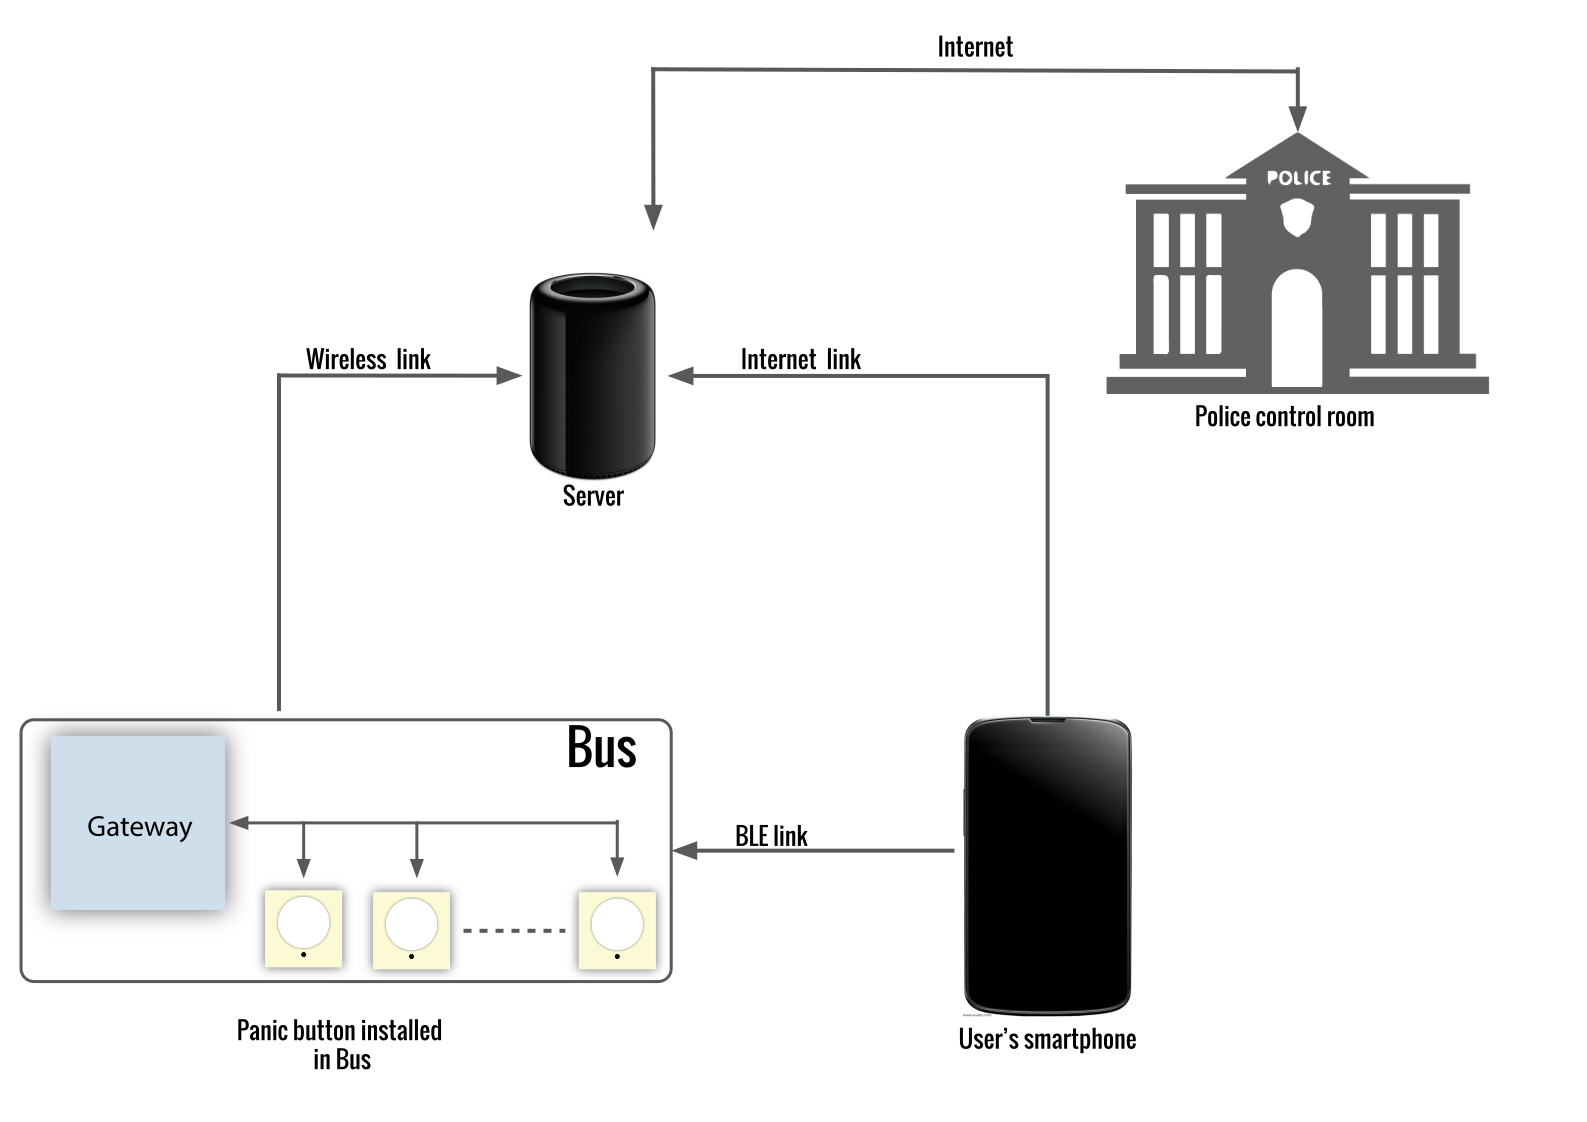
\includegraphics[width=0.9\textwidth]{bus}
\caption{Functional description of the \emph{PanicButton device} with audio-based trigger in bus}
  \label{fig:functionalDescbus}
\end{figure}

Emergency is asserted, if either the panic button is pressed or scream is detected by audio-based trigger. In case of emergency, compressed stream of audio along with vehicle's location is sent to the server, for later examination.


%This should include 
%\begin{itemize}
%\item a discussion on the product with the aid of block diagrams and figures
%\item an exhaustive list of stimuli to product
%\item classification of the stimuli as input/output, power signal/information
%signal, electric/mechanical etc.
%\item First level quantification of the stimuli like, voltage levels, type
%of signals (dc, ac, pulsed), rise time, current levels, etc.
%\end{itemize}

\section{Module study}
This section dwells in literature survey and design decision done for the individual modules.

\subsection{Protocols for communication}
We studied the protocols that can be used between the links present in the system. There are four different links in the system.
\begin{itemize}
\item link between the \emph{PanicButton device} and the back-end server,
\item link between the smartphone and the back-end server,
\item link between the smartphone and the \emph{PanicButton device},
\item link between the back-end server and the PCRs.
\end{itemize}
The following subsections will go into the details of each of them.
\subsubsection{Protocol for messaging between the \emph{PanicButton device}, the back-end server and PCRs}
The message link between panic button and back-end server must be a low latency link. In order to achieve that we looked at different protocols with their merits and demerits. The following protocols can be used for this link.
\begin{itemize}
\item Hypertext Transfer Protocol 1.1 (HTTP)
\item Message Queue Telemetry Transport (MQTT)
\item Constrained Application Protocol (CoAP)
\end{itemize} 
HTTP is one of most widely used protocol for data transfer. It is the foundation of data communication for the World Wide Web (WWW). HTTP is a text based application layer protocol, which uses Representation State Transfer (REST) with four methods \emph{GET}, \emph{PUT}, \emph{POST} and \emph{DELETE}.\\
MQTT is one of the emerging protocol in the Internet of Things(IoT) domain. MQTT uses Transmission Control Protocol(TCP) as transport layer. It uses publish subscribe pattern with only two methods \emph{SUBSCRIBE} and \emph{PUBLISH}. MQTT is a protocol with very small header overhead.\\
CoAP is another IoT protocol designed specifically to be used in the lightweight environments.  CoAP is designed to easily translate to HTTP for simplified intergration with the web. CoAP runs over User Datagram Protocol (UDP) transport layer.\\
Table~\ref{tab:mess_procotols} compares different protocols.
\begin{table}[H]
\begin{center}
\begin{tabular}{ |c|c|c|c|c| } 
 \hline
 \textbf{Protocol} & \textbf{REST/PubSub} & \textbf{Transport layer protocol} &\textbf{header} & \textbf{Min-header (bytes)} \\
 \hline 
 \hline
 HTTP & REST & TCP & Text & 18 \\
 \hline
 MQTT & PubSub & TCP & Binary & 2 \\ 
 \hline
 CoAP & REST & UDP & Text & 4  \\ 
 \hline
\end{tabular}
\end{center}
\caption{Camparision of HTTP, MQTT and CoAP} \label{tab:mess_procotols}
\end{table}
The architecture of the our system can benefit from publish subscribe model for transparent transfer of messages between the \emph{PanicButton device} and PCR, where back-end server will act as a message broker. The back-end server can relay messages transparently to different PCRs at different locations. MQTT uses binary header with smallest packet size of just 2 bytes, which helps in reducing the bandwidth requirement for the communication. 
\subsubsection{Protocol for audio streaming}
The audio stream link between the \emph{PanicButton device} and back-end server requires high throughput, low latency, guaranteed delivery link. The protocols under consideration are
\begin{itemize}
\item HTTP1.1 over TCP
\item Raw over TCP
\item Raw over UDP
\end{itemize}
We decided to use raw over TCP because it fulfills the requirements for this link. HTTP 1.1 also provides the same benefits as raw over TCP, but adds large header overhead which is not desired. The extra information regarding the stream can be embedded in the compressed audio stream explained in the next section.
\subsection{Compression algorithm}
\label{sec:compression}
The use of wireless link from the \emph{PanicButton device} to the back-end server restricts the bandwidth which is available for audio transmission. The compression of audio stream is essential for reliable transfer of audio from panic button to back-end server under congestion.\\

\begin{table}[H]
\begin{center}
\begin{tabular}{ |c|c|c|c| } 
 \hline
 \textbf{Format} & \textbf{Lossless} & \textbf{Compression factor} &\textbf{Open-source/royalty-free} \\
 \hline 
 \hline
 Raw & Yes &  1:1 & Yes\\
  \hline
 Wav & Yes &  1:1 & Yes\\
 \hline
 Mp3 & No &  5:1 & No\\
 \hline
 Vorbis Ogg & No &  10:1 & Yes\\
 \hline
\end{tabular}
\end{center}
\caption{Expermental comparision of different audio formats at 44100 sample rate and 16-bit per sample} \label{tab:audio_formats}
\end{table}
Different audio formats are experimentally compared in table~\ref{tab:audio_formats}. Vorbis is open-source, royalty free audio compression and streaming format. Vorbis ogg's performance is better compared to mp3 in terms of compression ratio. We decided to use Vorbis Ogg audio format for streaming audio from the \emph{PanicButton device} to the back-end server.
\subsection{Encryption algorithm}
%\subsubsection{Encryption between panic button and back-end server}
Encryption is used to avoid man-in-the-middle attacks between the  \emph{PanicButton device} and the back-end server. Two of the most popular encryption algorithms are Advanced Encryption Standard (AES) and RSA algorithm. RSA algorithm uses asymmetric key configuration, while AES algorithm uses symmetric key configuration. The advantage of using RSA algorithm over AES is that, even if public key(key stored in panic button) is compromised, the communication is not compromised.
We decided to use RSA over AES due to this advantage.
%\subsubsection{Encryption between enclosure tamper detection module and core-module}

%\subsection{System validation module}
%One of the most essential part of the system is to have a self check mechanism to ensure the full functioning of the system. In case an anomaly is found in the system, it should notify the user as well as the back-end server.\\
%The panic button is installed in the public transport which makes it very vulnerable to tampering. There are number of ways in which it can be tampered. Few of them are
%\begin{itemize}
%\item Removing the power source from the panic button.
%\item Tampering with the physical button.
%\item Tampering with the microphone.
%\item Tampering with the enclosure.
%\item Physically change in the circuit.
%\item Change in firmware of the micro-controllers.
%\item Replacing the entire system with a dummy one.
%\item Swapping two system with each other.
%\end{itemize}
%The system must be able to detect any kind of tampering, in order %to keep the trust intact with the users.\\
%We propose few tamper detection mechanisms, which can warn the %user while boarding.
%\subsubsection{Enclosure tamper detection}
%In order to detect tampering with the system, unauthorized access to internal circuitry and components must be detected. To handle this undesirable event we looked at following methods.
%\begin{itemize}
%\item An ultra low power push button based detection system, %which will change the state of button if somebody tries to open %the enclosure.
%\item An ultra low power wire based detection system, which will %break if somebody tries to open the enclosure.
%\end{itemize}
%In push button based detection system, push button will be %installed inside the enclosure, which will be enabled as soon as %enclosure opens.\\
%In wire based detection system, wire runs around the periphery of %the enclosure, which will permanently break as soon as enclosure %opens.\\
%Tamper detection module must be always-on, independent of the %power source availability. It must have battery life of atleast %few years for tamper detection to work reliably.\\
%The tamper detection module must retain state independent of %change the firmware or change of the component. In order to %achieve that the core-module must detect that change. We propose %to store secret private key in tamper detection module and core-%module. The communication between the core-module is encrypted so %that third party can't watch the exchange of messages. In case of %tamper, tamper detection module permanently deletes his copy of %private key.\\
%Advanced Encryption Standard (AES) algorithm is not appropriate %for ultra low power microcontroller. A tiny footprint encryption %algorithm is required to encrypt the messages transfered between %core-module and tamper detection module.\\
%Tiny Encryption Algorithm (TEA) is a encryption algorithm %suitable for ultra low power microcontroller. Instead to relying %on complicated operation, it uses large number of iterations of %simple operations\cite{tea_paper}. We used Modified Tiny %Encryption Algorithm (MTEA), which is based on TEA with 16-bit %operations instead of 32-bit operations.
  



\subsection{Audio-based trigger module}
This audio-based trigger comes under \emph{sound event detection} domain of relatively broad research area of audio/sound analysis. Sound event detection is relatively new area compared to speech analysis, so most of the literature in the field of acoustic analysis is highly clustered around speech analysis. In section~\ref{sssec:featforscream}, we take a look at literature survey and experiments done to come up with required feature for scream detection; in section~\ref{sssec:algoforscream}, we take a look at literature survey done for algorithm to be used for scream detection.

\subsubsection{Feature for scream detection}
\label{sssec:featforscream}
Features extracted from acoustic signals are vectors that can faithfully represent them. In order to develop the best possible classification algorithm for reliable detection and classification of sound events, it is very important to select the feature set carefully. Although a large feature set has its benefits of generating accurate results, using a small feature set can reduce latency and make the design simpler.

Over the last few years, several audio feature extraction techniques have been introduced. They make use of one of the following two signal representation domains: temporal
and spectral. Temporal domain features such as signal energy, pitch, zero-crossing \cite{paper4} rate and entropy modulation \cite{paper5} have been used for speech classification but are not enough to represent the non-stationary characteristics of sound events. Spectral features such as percentage of low energy frames, 4-Hz modulation energy, spectral roll-off point, mean frequency, spectral centroid, mel-frequency cepstral coefficients and frequency slopes are useful in audio classification, but they do not provide any information about the temporal evolution of the extracted features over the frame.

Initially researchers used popular mel-frequency cepstral coefficients (MFCC) as features for sound event detection. MFCC are short-term spectral based features. These features are extracted through a series of digital signal processing steps like windowing, Discrete Fourier Transform(DFT), logarithm and Discrete Cosine Transform (DCT). MFCC are still used for non-verbal sound recognition \cite{paper6}. A paper\cite{paper7} proposed a sound event classifier which use MFCC feature set; they achieved 74\% accuracy. Another paper \cite{paper8} successfully classified acoustic environmental sounds like office, soccer match, beach, laundrette, street noise, rail station, car, bar and bus using a Hidden Markov Model(HMM) based classifier which used MFCC as feature vectors.

%TODO ref for LPC
Linear predictive coefficients (LPC) is another well known feature set used for sound
classification of car noise, factory noise, street noise, babble and bus noise. A Quadratic
Gaussian classifier using LPC feature set gives accuracy of 90\% for car/factory noise
and 60-80\% for the rest.

Time-Frequency Matrix(TFM) feature set tends to capture non-stationary and discontinuous properties of sound events. This matrix is obtained using matching-pursuit time-frequency distribution (MP-TFD) technique, followed by non-negative matrix decomposition to decompose the TFM into its significant components \cite{paper9}.

After looking at individual feature sets, researchers started fusion of various feature sets. \cite{paper6} used MFCC along with Pitch range based features, \cite{paper10} used MFCC along with spectral features like centroid, flux, flatness, roll-off, harmonic-to-noise ratio and pitch. TFM when combined with a few spectral and MFCC features, gives 10\% accuracy-rate improvement compared to only MFCC features based classifiers \cite{paper9}.

One paper \cite{paper11} went in completely different direction to tackle the issue of sound event classification, they argued that sound events produced a unique texture, which can be visualized using a spectrogram image and could be analyzed for automatic sound event detection. Another paper \cite{paper12} used pseudo-coloration to enhance the perception. Spectrogram is first normalized into grey-scale with a fixed range, then dynamic range is quantized in to regions, each of which is then mapped to form a monochrome image. Finally monochrome images are partitioned in to blocks and distribution statistics in each block are extracted to form the feature set. Robustness of spectrogram based methods comes from the fact that noise
is normally more diffused than the signal and therefore the effect of noise is limited to a
particular quantization region, leaving other regions less effected.

Feature used in detection/classification systems impacts their response time and power
consumption. A non-realtime application can make use of large and time consuming feature sets to get highly accurate results, while a realtime application can only use feature
set that fit into its time budget. Power consumption is important aspect in battery powered devices; Feature set that can give acceptable accuracy at lesser computation results in system that lasts longer on a single charge.

We decided to use MFCC along with spectral features like centroid, flux, flatness, roll-off, harmonics-to-noise ratio and pitch due to its promising performance \cite{paper10}. We conducted an experiment to find out the execution time of this feature set. The task of detecting scream is to be performed in real-time. In our project we decided to analyze live audio stream every 1 second, which gives us 2 second to analyze and give results for audio received in previous second, this decision was based on the analysis done by \cite{paper10}, which showed average scream duration to be around 2 second. We tried MFCC plus few spectral features as feature vector and computed feature extraction time for an audio clip of 2 second, Table~\ref{tab:scr2} summarizes scream detection time on two hardwares.

\begin{table}[H]
\begin{center}
\begin{tabular}{ |c|c| } 
 \hline
 \textbf{Platform} & \textbf{Feature extraction time (in s)} \\
 \hline 
 \hline
 Raspberry pi 3 & 13 \\
 \hline
 Intel quad core i5-4440 @ 3.10GHz (16 GB) & 1.5 to 2 \\ 
 \hline
\end{tabular}
\end{center}
\caption{Feature extraction time using MFCC and spectral feature as feature vector} \label{tab:scr2}
\end{table}

With MFCC and spectral features as feature set, we had latency of 13 sec which is beyond the 2 sec limit. We had to shed computationally expensive part of this composite dataset to squeeze into the budget of 2 sec, we decided to use only MFCC as feature vector and Table~\ref{tab:scr1} summarizes the execution time of this dataset.

\begin{table}[H]
\begin{center}
\begin{tabular}{ |c|c| } 
 \hline
 \textbf{Platform} & \textbf{Feature extraction time (in s)} \\
 \hline 
 \hline
 Raspberry pi 3 & 1.480 \\
 \hline
 Intel quad core i5-4440 @ 3.10GHz (16 GB) & 1.020 to 1.050 \\ 
 \hline
\end{tabular}
\end{center}
\caption{Feature extraction time using MFCC as feature vector} \label{tab:scr1}
\end{table}

With MFCC as feature vector we have latency of 1.480 sec, which is less than our time limit of 2 sec. We decided to go with MFCC as the feature vector for scream detection.

\subsubsection{Classification algorithm for scream detection}
\label{sssec:algoforscream} 

These algorithms take features as input and output probabilities of all classification class for the given input. The class with highest probability for a given input is said to be the class of the input.

Initially researchers used classifiers like a quadratic Gaussian classifier, a least-square
linear classifier, a neighbor classifier and a decision tree classifier \cite{paper6}. These classifiers could preform well for particular sound events but couldn't generalize well to non-verbal sound events.

Lately researches have started using machine learning for the purpose of sound event classification. Algorithms like Artificial Neural Network (ANN) \cite{paper6} and Support Vector Machine(SVM) \cite{paper10} are being used widely. These algorithms fall under the category of supervised machine learning. These algorithms outperform nearly all other classifiers used in past due to their capability to model complex systems.

ANNs are mathematical models that emulates biology of a human brain. ANNs are parallel computing mechanisms that contains neurons laid out as a layers, interconnects and learning rules. SVMs are another set of mathematical models used for classification. SVMs constructs a hyperplane or set of hyperplanes in a high dimensional space, which is used for classification. ANN algorithms require more data to train the classifier as compared to SVMs. In case of SVMs, we need to set a limited number of parameters and choose among possible kernel. We decided to use SVM algorithm due to available limited dataset and easy convergence in training. 

%For each of the modules, include
%\begin{itemize}
%\item an exhaustive list of stimuli to the module
%\item classification of the stimuli as input/output, power signal/information
%signal, electric/mechanical etc.
%\item First level quantification of the stimuli like, voltage levels, type
%of signals (dc, ac, pulsed), rise time, current levels, etc.
%\end{itemize}

%\subsection{Sub-modules}

%If necessary, partition the various modules into sub-modules and %so
%on till the component level. 

%\emph{NOTE}: At every module, sub-module or component level (electric
%hardware or algorithms or industrial design), if there are multiple
%options available, then perform a comparative study of the most significant
%features among the options to evaluate the merits and demerits of
%the various options. Based on the merits and demerits of the various
%options, give your recommendations for design.


\section{Industrial design}
Being a product for public safety service, it should blend with the vehicular environment yet remain accessible. The panic button mounted on the \emph{PanicButton device} has to be easily accessible 24x7. A button with area equal to the average area of adult hand and back-light will fulfill these requirements. Front panel of the \emph{PanicButton device} mounts three essential part namely panic button with status back-light, speaker and microphone. Front panel also acts as lid for the \emph{PanicButton device}. Secondary battery and electronics used in this project resides at the base of enclosure. Figure~\ref{fig:baselayout} shows a pictorial representation of the assembly.

\begin{figure}[H]
\centering
\includegraphics[width=\textwidth]{base_layout}
\caption{Layout of battery and electronics at the base of the \emph{PanicButton device}}
\label{fig:baselayout}
\end{figure}  

Details of this enclosure will be covered in Industrial design section of chapter 3.


%The industrial design/product design aspects should consider the following,
%\begin{itemize}
%\item Design mix - functional, ergonomics and aesthetics aspects of the
%product should be discussed giving consideration to appropriateness
%to a given application.
%\item Layout - the layout of the modules and the sub-modules within an enclosure
%or system should be discussed as determined by the following considerations, 

%\begin{itemize}
%\item user, form, ergonomics, aesthetics, interconnections, display, etc.
%\item realisation issues of a particular layout
%\item functional aspects like EMI, thermal, wiring etc.
%\end{itemize}
%\item Product structure - provide a discussion on the product generic structure,
%whether it should be

%\begin{itemize}
%\item rack and frame mounted 
%\item modular cabinet
%\item non-modular
%\item custom 
%\end{itemize}
%\item Materials - provide a discussion on the choice of materials for the
%product
%\item Manufacturing processes
%\item Cost of the product
%\end{itemize}

%\section{Target scope}

%The following questions need to be addressed:
%\begin{itemize}
%\item What is the targetted scope of the product?
%\item What is the set of target specifications to design the product?\end{itemize}

\chapter{Design}
In this chapter, we dwell into the detailed design of the project. Section~\ref{sec:module} lists the individual modules designed in this project. Section~\ref{sec:hardware} gets into details of all the hardware design; section~\ref{sec:software} does the same for software design. Finally section~\ref{sec:desIndust} dwells into details of industrial design of the project.
\begin{figure}[H]
\centering
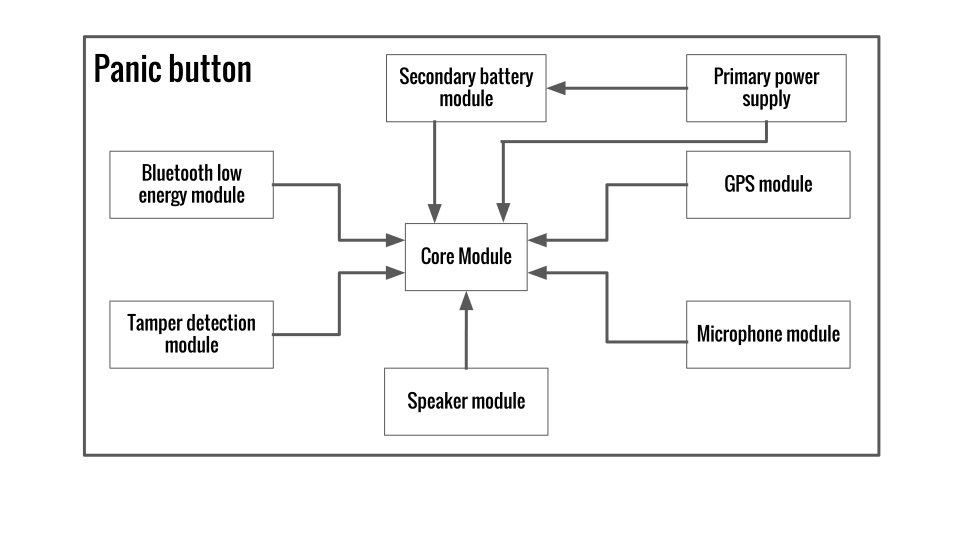
\includegraphics[width=\textwidth]{block_dia}
\caption{Block diagram of the \emph{PanicButton device}}
\label{fig:block_dia}
\end{figure}

%The chapter includes
%\begin{itemize}
%\item design of modules and sub-modules
%\item design equations (with electrical and thermal stresses)
%\item component selection
%\item design of algorithms
%\item industrial design aspects
%\item system integration issues
%\end{itemize}

\section{Module partitioning}
\label{sec:module}
This section gives an overview for the content in next two sections. Section~\ref{sec:hardware} describes the design of hardware used in the project. It is divided in three major sections-
\begin{itemize}
\item \emph{PanicButton device}- describes the design of core module, tamper detection module, etc.
\item Server- describes the hardware involved in server and,
\item Smartphone- describes the hardware involved in smartphone.
\end{itemize}

Section~\ref{sec:software}, describes the design of the firmware used in the project. This section dwell in to the software design aspects of-
\begin{itemize}
\item System validation module,
\item Audio streaming module,
\item Global Positioning System module,
\item Panic button module and,
\item Audio-based trigger module.
\end{itemize}  
 
%Based on the module and sub-module partitioning of the previous chapter
%\begin{itemize}
%\item the segregation of modules into hardware, embedded software and standalone
%software parts
%\item the exhaustive list of stimuli to the modules (hardware and software)
%\item detailed quantification of the stimuli for both hardware and software
%modules
%\end{itemize}

\section{Hardware design}
\label{sec:hardware}
\subsection{\emph{PanicButton device}}
\subsubsection{Core-module}
The core-module for the system is based on Raspberry pi 3. Raspberry pi uses BCM2837 SOC from Broadcom, with four ARM Cortex-A53 64-bit cores running at 1.2GHz, a Broadcom VideoCore IV Graphics Processing Unit (GPU), 1 GB LPDDR2 Random access Memory (RAM) which runs at 900MHz, 10/100 Ethernet, 2.4GHz 802.11n Wireless Fidelity (WiFi) and micro secure digital (microSD) card with maximum size of 128 GB. Peripherals connects to a High-Definition Multimedia Interface (HDMI) port, four Universal Serial Bus (USB) 2.0 ports, one audio-video port, Camera Serial Interface (CSI) and Display Serial Interface (DSI) available on board.
Raspberry pi 3 has a 40-pin Header, which contains one Serial peripheral interface (SPI) with two chip select pins, one Inter-integrated Circuits (I2C), one Universal Asynchronous Receiver Transmitter (UART) and 18 General Purpose Input Output (GPIO) pins.
The schematic of the core-module is shown in figure~\ref{fig:core_module_sch}.
\begin{figure}[H]
\centering
\includegraphics[height=10cm]{core_module_sch}
\caption{Schematic of the core-module of the \emph{PanicButton device}}
\label{fig:core_module_sch}
\end{figure}


\subsubsection{Tamper detection module}
The \emph{PanicButton device} is installed in public transport, which makes it very vulnerable to tampering. In order to tamper with the device, they must first open the enclosure. The tamper detection module detects opening of the lit/top panel by using a switch and stores that information in non-volatile memory. The normally closed type switch is connected between the base of enclosure and the top lid; It changes its state when lid is opened. The tamper detection module uses an ultra lower power MSP430G2553 microcontroller running on CR2032 Lithium ion coin cell auxiliary battery. SPI interface is used to communicate between the microcontroller and the core-module.
\begin{figure}[H]
\includegraphics[width=\textwidth]{tamperingproofsytem_sch}
\caption{Schematic of Tamper detection module}
\label{fig:tamperingproofsytem_sch}
\end{figure}

\subsubsection{Panic button \& LED drive module}
Panic button is a normally open non-latching type switch with 10 kOhm pull resistor which pulls it up to 3.3 V. A 2N4401 transistor is used in parallel with the switch to emulate the switch press to test the functioning of the switch. 100 kOhm resistor connected to the base terminal of the transistor, limits the current flowing through the base and emitter terminals. \textit{B\_TEST} is output from core-module and \textit{P\_BUTTON} is input to the core-module.
Two 2N4401 are used to drive four red and four green LEDs for status indication. \textit{R\_LED} and \textit{G\_LED} are output from the core-module to drive these LEDs. The schematic of module is shown in figure~\ref{fig:pbutton_sch}.
\begin{figure}[H]
\begin{subfigure}{.5\textwidth}
  \centering
  \includegraphics[width=.95\linewidth]{pbutton_sch}
  \caption{}
  \label{fig:p_button_a}
\end{subfigure}%
\begin{subfigure}{.5\textwidth}
  \centering
  \includegraphics[width=.95\linewidth]{rg_led}
  \caption{}
  \label{fig:p_button_b}
\end{subfigure}
\caption{Schematic of (a) LED driver (b) Panic button}
\label{fig:pbutton_sch}
\end{figure}

\subsubsection{GPS module}
The Global Positioning System (GPS) module is NEO-6M module from Ublox. NEO-6M uses AssistNow Autonomous Technology,  which provides functionality similar to Assisted GPS (A-GPS) without the need of external network connection. Based on previously broadcast satellite ephemeris data downloaded to and stored by the GPS receiver. AssistNow Autonomous Technology generates accurate satellite orbital data(``AssistNow Autonomous data") that is used for the future GPS position fixes. Electrically Erasable Programmable Read-Only Memory (EEPROM) is used to store parametric data of GPS receiver (NEO-6M).
UART protocol is used to connect GPS module to the core-module as shown in figure~\ref{fig:gps_sch}.    % NEO-6M uses aiding information like ephemeris, almanac, rough last position and time and satellite status and an optional time synchronous signal to reduce time to first fix significantly and improve the acquisition sensitivity.
\begin{figure}[H]
\includegraphics[width=\textwidth]{gps_sch}
\caption{Schematic of GPS module}
\label{fig:gps_sch}
\end{figure}

\subsubsection{Bluetooth low energy module}
The Bluetooth Low Energy (BLE) module uses nRF51822QFAC SOC from Nordic Semiconductors. nRF51822 SOC has ARM\textsuperscript{\textregistered} Cortex\textsuperscript{\texttrademark}-M0 32-bit processor running at 16 MHz with 256 kB of embedded flash program memory and 32 kB of RAM. It requires one crystal for system clock and one 32.768 kHz crystal for real time clock functionality. It uses 50 $\Omega$ impedance matching circuit for maximum radiation as shown in right hand side of figure~\ref{fig:ble_sch}.\\
4-wire SPI interface is used to connect the SOC to the core-module. 
\begin{figure}[H]
\includegraphics[width=\textwidth]{ble_sch}
\caption{Schematic of Bluetooth low energy module}
\label{fig:ble_sch}
\end{figure}

\subsubsection{Speaker module}
A 8 $\Omega$ 0.5 watt speaker and microphone pair is used to validate the microphone in a closed loop. As core-module cannot drive the 8 $\Omega$ speaker directly, we designed LM386 Integrated Circuit (IC) based amplifier to drive the speaker. A 10 k$\Omega$ potentiometer is used in series with 10 uF bypass capacitor to adjust the gain manually as shown in figure~\ref{fig:speaker_amp_sch}.
\begin{figure}[H]
\includegraphics[width=\textwidth]{speaker_amp_sch}
\caption{Schematic of speaker amplifier module schematic}
\label{fig:speaker_amp_sch}
\end{figure}

\subsubsection{Microphone module}
Core-module does not have an on-board audio input support. We used external USB sound-card to add audio input(microphone) to the core-module as shown in the figure~\ref{fig:audio_trigger_sch}.% The sound-card measured 11.2 x 8.4 x 2.1 cm and weighed 82 grams. An omni-directional microphone gets connected at the input port of the sound card. Hardware for audio-based trigger is shown in figure~\ref{fig:audio_trigger_sch}.
\begin{figure}[H]
\includegraphics[width=\textwidth]{audio_trigger_sch}
\caption{Schematic for microphone module}
\label{fig:audio_trigger_sch}
\end{figure}

\subsection{Back-end server}
We used a desktop computer as the back-end sever with specification given below.
\begin{itemize}
\item \textbf{Processor:} Intel\textsuperscript{\textregistered} Core\textsuperscript{\texttrademark} i5-4440 quadcore processor running at 3.1 GHz.
\item \textbf{Graphics processor:} Integrated Intel\textsuperscript{\textregistered} HD Graphics 4600 running at 350 MHz.
\item \textbf{RAM:} Kingston value RAM 16 GB DDR3 running at 1600 MHz.
\item \textbf{Hard disk:} Seagate SATA SSHD 1 TB desktop internal hard drive 7200RPM.
\end{itemize}

\subsection{Smartphone}
We used a Google Nexus 4 smartphone running Android 5.1.1 to test designed application. The specification of the smartphone are given below. 
\begin{itemize}
\item \textbf{SOC:} Qualcomm APQ8064 Snapdragon S4 Pro with four Krait running at 1.5 GHz and Adreno 320 GPU running at 400 MHz.
\item \textbf{Radio:} Wi-Fi 802.11 a/b/g/n and Bluetooth v4.0.
\item \textbf{Battery:} 2100 mAh.
\item \textbf{Screen:} 4.7 inches 768 x 1280 pixels In-Plane Switching (IPS) display.
\end{itemize}

\emph{Note: Any smartphone with Bluetooth v4.0 or above and running Android 4.3 or above can be used.}

%Based on the stimuli classification of each module or sub-module,
%perform the design which includes
%\begin{itemize}
%\item the final circuit schematic
%\item design equations relating to functional aspects like accuracy, resolution,
%dynamics and harmonics with respect to the output
%\item design equations relating to electrical stresses of components or
%devices
%\item design equations relating to thermal stresses of components or devices
%\item selection of devices based on the design equations
%\item selection of associated non-electrical parameters and components like
%heat sink, wires, connectors, switches etc.
%\item reliability estimate in terms of mean time to failure (MTTF)
%\end{itemize}
%NOTE: \emph{include as many sections/sub-sections as there are hardware
%modules/sub-modules and repeat the above for every hardware module
%and sub-module}.


\section{Software design}
\label{sec:software}
\subsection{System validation module}
The system validation module is responsible for self checking and notifying the user about the status of the system. The system validation module tests the microphone, panic button, firmware and enclosure tamper state.\\
The microphone and panic button validation runs every time a new user boards the vehicle or a user wants to re-validate the system. The microphone and the panic button has a five second timeout period after which the validation state is invalidated. The firmware validation is done after every reset and it doesn't have a timeout period. The enclosure tamper detection is an always-on validation sequence, which syncs its state every minute with tamper detection hardware.\\   
The flow chart of system validation procedure is shown in figure~\ref{fig:ble_validation}. \\
The components involved in the validation of the system are as follows.
\begin{itemize}
\item User's smartphone
\item nRF51822 BLE SOC
\item Core-module
\item Server
\end{itemize}
User's smartphone connects to the nRF51822 and sends a random \emph{connectionID} to it and closes the connection. User's smartphone waits for the response from the server. The nRF51822 relays the \emph{connectionID} to the core-module. Core-module checks whether the previous validation results are still valid. If it is not valid, then core-module will start the validation sequence to validate the state of the system. If the previous validation results are valid or the current validation sequence completes, then core-module sends the validation results, \emph{connectionID}, \emph{date-time} and encrypted \emph{panicButtonID} to the server. If the server finds the \emph{panicButtonID} in the database, then it sends the driver details, vehicle details and validation results to the user's smartphone. The user's smartphone will show a notification to interrupt the user, which contains the information received from the server.\\
The flowchart of the system validation module is shown in figure~\ref{fig:ble_validation}.
Next we will look into the working of individual components.
\begin{figure}[H]
\centering
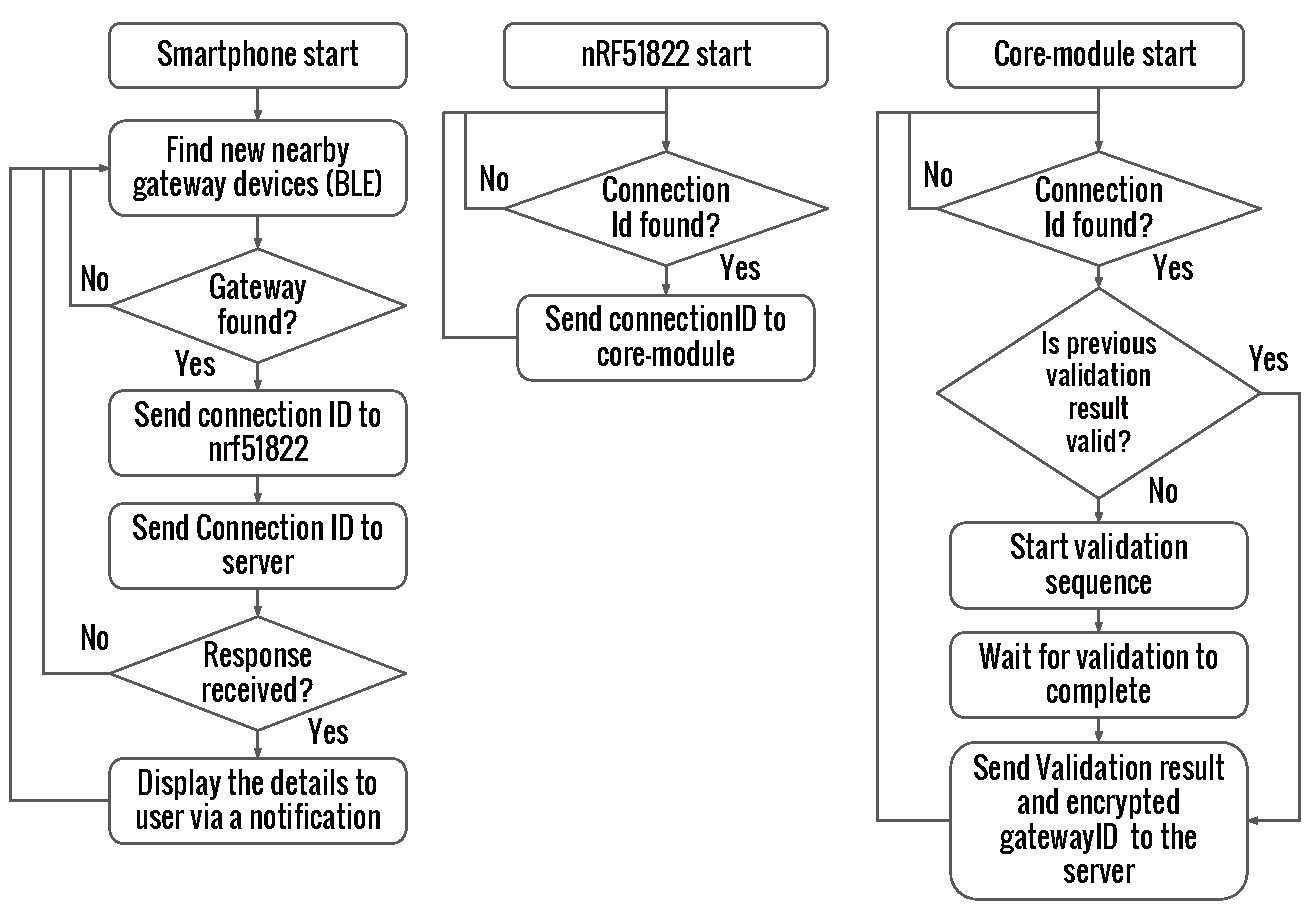
\includegraphics[width=\textwidth]{ble_validation.pdf}
\caption{Flow chart for BLE system validation module}
\label{fig:ble_validation}
\end{figure}
\textbf{nRF51822}
acts as a relay between core-module and user's smartphone. nRF58122 uses Generic Access Profile (GAP) to control the connections and advertising. BLE's GAP layer is responsible to broadcast connectible beacons to show \emph{PanicButton device}'s presence to the nearby devices for them to connect.\\
nRF51822 is running a Generic Attribute Profile (GATT) server to serve the validation service with \emph{connID} characteristic. The UUID used are shown in table~\ref{tab:Ids}.

\begin{table}[H]
\begin{center}
\begin{tabular}{ |c|c| } 
 \hline
 \textbf{} & \textbf{UUID}\\
 \hline 
 \hline
  Validation service & 6E400001-B5A3-F393-E0A9-E50E24DCCA9E\\ 
 \hline
 \emph{ConnID} characteristic & 6E400002-B5A3-F393-E0A9-E50E2DCCA9E \\ 
 \hline
\end{tabular}
\end{center}
\caption{UUIDs of the BLE services} 
\label{tab:Ids}
\end{table}

%\begin{itemize}
%\item \textbf{Validation service} 6E400001-B5A3-F393-E0A9-E50E24DCCA9E
%\item \textbf{\emph{ConnID} characteristic} 6E400002-B5A3-F393-E0A9-E50E2DCCA9E
%\end{itemize}
nRF51822 forwards the \emph{connectionID} received from user's smartphone  to the core-module using SPI protocol.

\textbf{Android app} runs on user's smartphone as a background service to scan for nearby \emph{PanicButton devices}. App differentiates the \emph{PanicButton device} from other devices using services they offer i.e., if some device has the service and characteristics IDs as mentioned in table~\ref{tab:Ids}, it considers the device as a valid \emph{PanicButton device}.\\
As soon as a valid \emph{PanicButton device} is found, the app connects to the \emph{PanicButton device} and sends a pseudo random 32-bit number to it and disconnects. After disconnection from the \emph{PanicButton device}, app sends the same number to the server and waits for server's response. Once the server's response is received, app builds a notification with information received from server and display it to the user. In case the validation of the \emph{PanicButton device} is successful, it will display ``Welcome, safe to enter", otherwise it will display ``Caution, enter at your own risk". The screeshots of the android app is shown in figure~\ref{fig:android_screenshot}. 

\begin{figure}[H]
\begin{subfigure}{.5\textwidth}
  \centering
  \includegraphics[width=.9\linewidth]{android_safe}
  \caption{Screenshot of ``Welcome, safe to enter"}
  \label{fig:android_safe}
\end{subfigure}%
\begin{subfigure}{.5\textwidth}
  \centering
  \includegraphics[width=.9\linewidth]{android_caution}
  \caption{Screenshot of ``Caution, enter at your own risk"}
  \label{fig:android_caution}
\end{subfigure}
\caption{Screenshots of Android app}
\label{fig:android_screenshot}
\end{figure}



\textbf{Core-module} receives \emph{connectionID}, when a user's smartphone connects to nRF51822. The core-module will add the \emph{connectionID} to the queue of \emph{connectionIDs}. Each \emph{PanicButton device} has it own unique and secret 128-bit  \emph{panicButtonID} stored in the core-module associated with it, embedded in the non-volatile memory. The \emph{panicButtonID} is used to validate the identity of the \emph{PanicButton device} to the server.
After receving the \emph{connectionID} for the user's smartphone, the core-module will start a new validation sequence if the previous validation result is not valid anymore due to timeout event. Once a valid validation result is ready, the core-module will merge \emph{connectionID} and \emph{panicButtonID} into \emph{mergedID}. The data flow for merging the IDs is shown in figure~\ref{fig:merged_id}.
\begin{figure}[H]
\centering
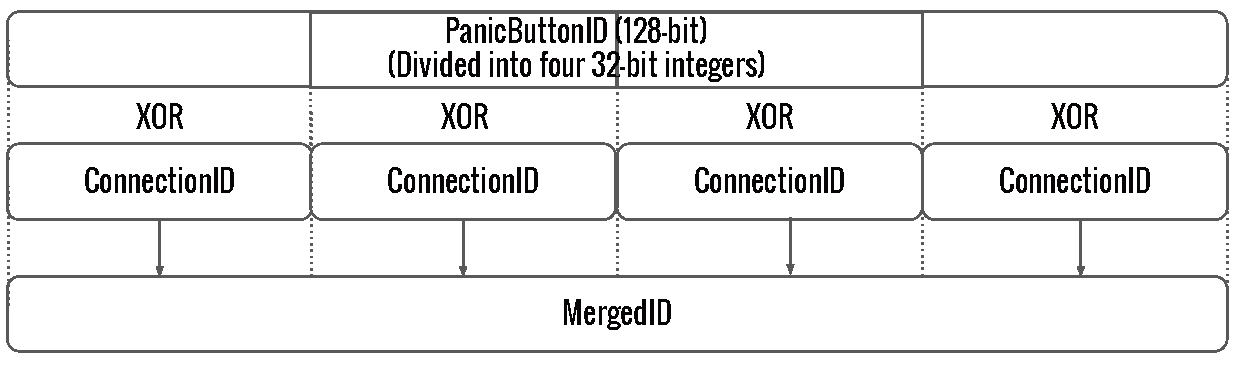
\includegraphics[scale=0.7]{merged_id.pdf}
\caption{Data flow for merging the connectionId and panicButtonID}
\label{fig:merged_id}
\end{figure}
\emph{MergedID} is encrypted to get \emph{cipherCode} by RSA algorithm using 256-bit public encryption key, which is stored in non-volatile memory of core-module.\\
The core-module will send Message Queuing Telemetry Transport (MQTT) message to \emph{``/gateway/validation"} topic in JavaScript Object Notation (JSON) format containing \emph{connectionID}, \emph{cipherCode}, \emph{date-time} and \emph{validationResult} fields.

\begin{figure}[H]
\centering
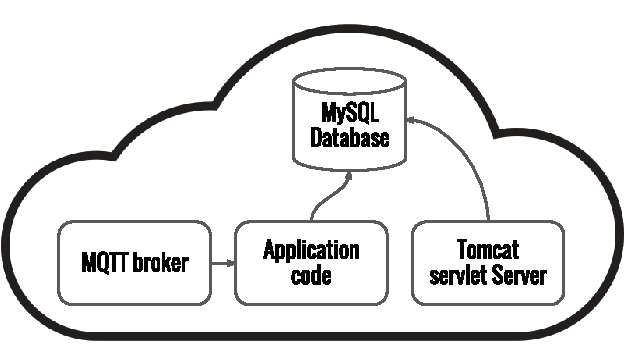
\includegraphics[]{server.pdf}
\caption{Overview of server running in the cloud}
\label{fig:server}
\end{figure}

\textbf{Server} is running a MQTT broker, a Tomcat servlet server, a MySQL database and application code to handle incoming MQTT messages as shown in figure~\ref{fig:server}.\\
Server is connected to the MySQL database, which has information of all the gateways \emph{PanicButton devices} and the vehicles. When a user's smartphone connects to server, it sends a unique random 32-bit \emph{connectionID}. When the \emph{PanicButton device} sends the validation results, it also sends the \emph{connectionID} to the server. The \emph{connectionID} is used to match the two connections (MQTT from \emph{PanicButton device} side and HTTP from smartphone side). Server waits for both connection to be established to synchronize the processing of the validation request.
 
The server holds the connection from user's smartphone until, it receives the same \emph{connectionId} in MQTT message in topic \emph{``/gateway/validation"} from \emph{PanicButton device}. Once the synchronization completes, the server decrypts the \emph{panicButtonID} using the secure private key stored in it. If the \emph{panicButtonID} exists in the database, the server sends the details to the smartphone or else it sends a NULL object to the smartphone. Server also sends validation results and date-time to the user's smartphone in JSON format. After sending the data, server closes the connection.\\


Next we will look into individual modules that gets validated.

\subsubsection{Microphone validation}
Microphone is one the most important module in the system. To Validate the microphone functionality, we are using a closed loop validation procedure as shown in figure~\ref{fig:mic_validation}.
\begin{figure}[H]
\centering
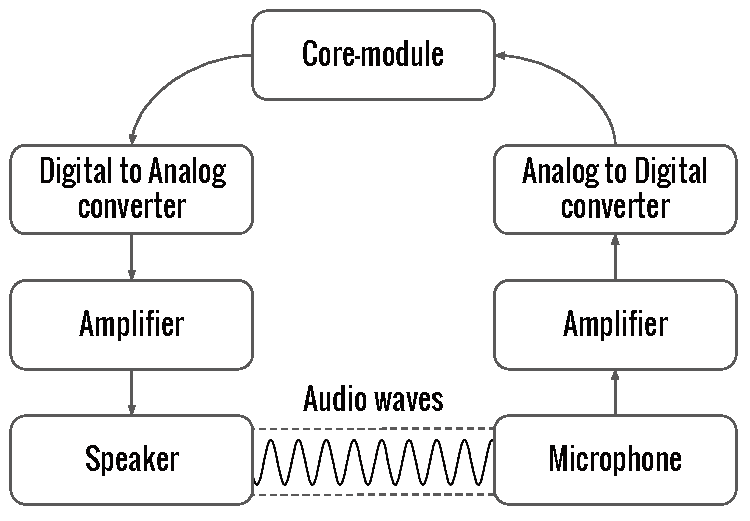
\includegraphics[scale=1]{mic_validation.pdf}
\caption{Microphone validation procedure}
\label{fig:mic_validation}
\end{figure}
Core-module generates a stream of pulsed single tone audio which corresponds to binary code of 10100101 and single tone frequency of 19 kHz as shown in figure~\ref{fig:waveform}.\\
\begin{figure}[H]
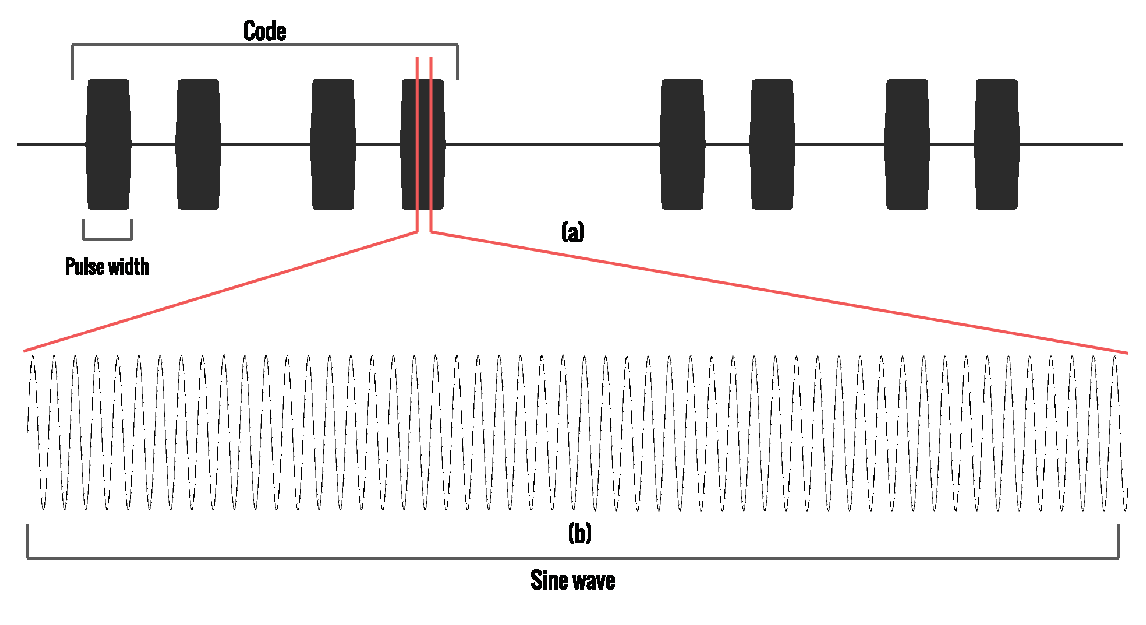
\includegraphics[width=\textwidth]{waveform.pdf}
\caption{Waveform of pulse single tone audio data (a) code sent via speaker (10100101) (b) sine wave of frequency 19000kHz}
\label{fig:waveform}
\end{figure}
\paragraph{Validation sequence\\}
For the validation of the microphone, we need two threads. First thread generates the audio stream and play it on the speaker and second thread analyses the audio stream received from the microphone to validate the microphone.\\
%subparagraph{Speaker Thread}
\textbf{Speaker thread} initializes the speaker to the default state and drains the existing audio date from the stream. Rise time of the waveform is not infinite, instead it rises slowly and linearly from zero to full amplitude in 3 ms. This helps in reducing high frequency harmonics. The audio data shown in figure~\ref{fig:waveform} is played through the speaker. After this operation, the speaker thread is suspended.\\
%\subparagraph{Microphone Thread}
\textbf{Microphone thread} initializes the microphone to the default state and flushes the existing audio data from the stream. Microphone waits for 441 samples to perform 441 point FFT. After calculating FFT, power around 19 kHz is calculated. The power calculated is then added to the time series queue of 50 samples, where the oldest power points are discarded. The \emph{correlation} is calculated for received time-series with the original data sent from the speaker. If the \emph{correlation} value exceeds the defined threshold then validation passes or else the process repeats until the timeout occurs. After the timeout it will retry microphone validation for two more times. If even after third try, the timeout occurs then validation is considered to be failed. The algorithm is explained in the flowchart shown in the figure~\ref{fig:mic_validation_flowchart}.
\begin{figure}[H]
\centering
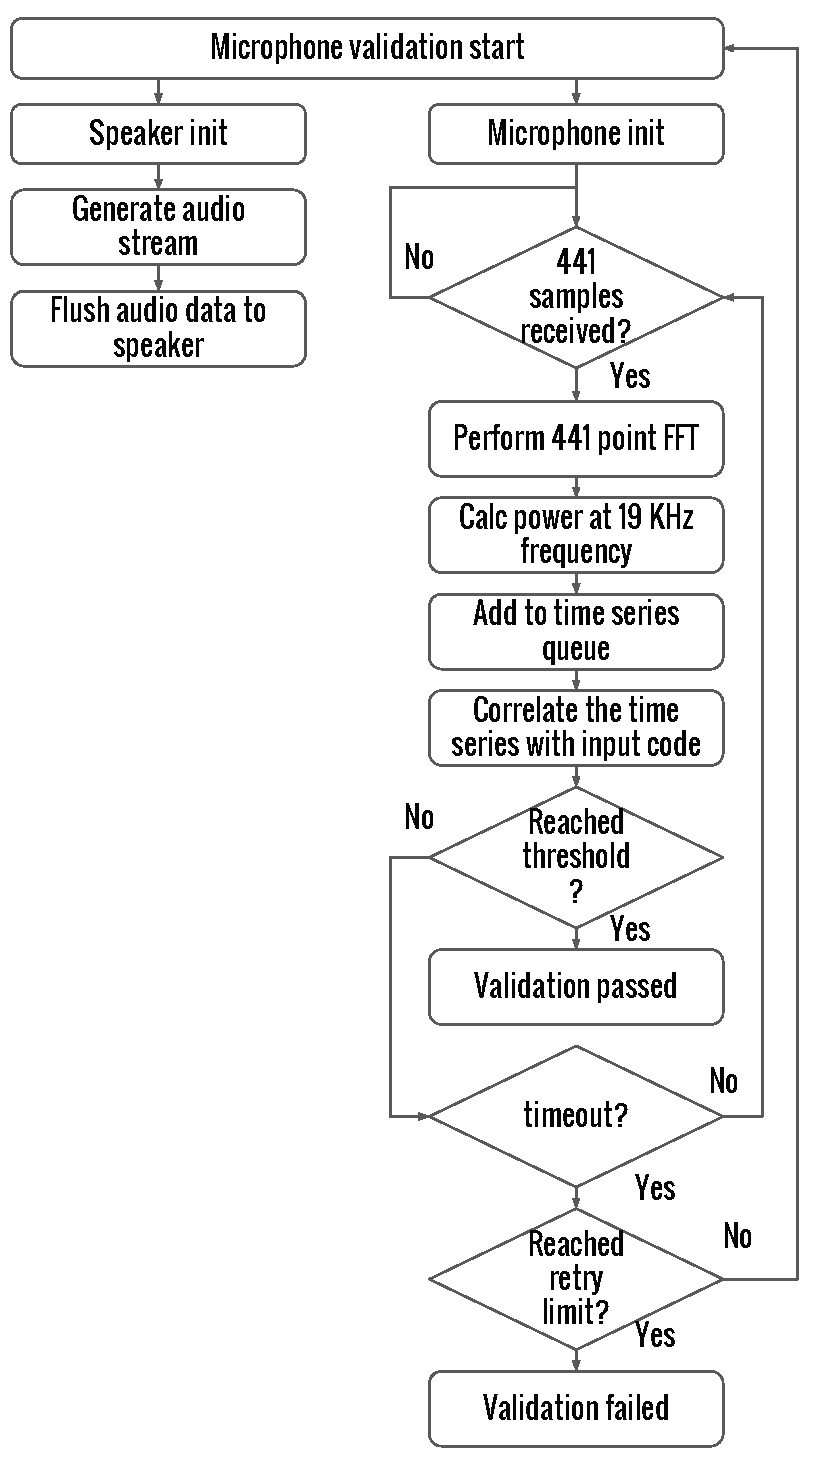
\includegraphics[width=0.7\textwidth]{mic_validation_flowchart.pdf}
\caption{Flow chart of microphone validation procedure}
\label{fig:mic_validation_flowchart}
\end{figure}
\subsubsection{Panic Button validation}
To validate the panic button, we emulate button press by shorting the pins of panic button by using the transistor as a switch, shown in figure~\ref{fig:p_button_a}. First the initial condition is tested for open. If the test passes then transistor pin is set to emulate button press. Second condition is tested for short. If the test passes then the validation succeeds. The transistor pin is reset which emulates button release. If any test fails then it will retry the procedure two more times. If even after third try, the test still fails then validation is considered to be failed. 
\begin{figure}[H]
\centering
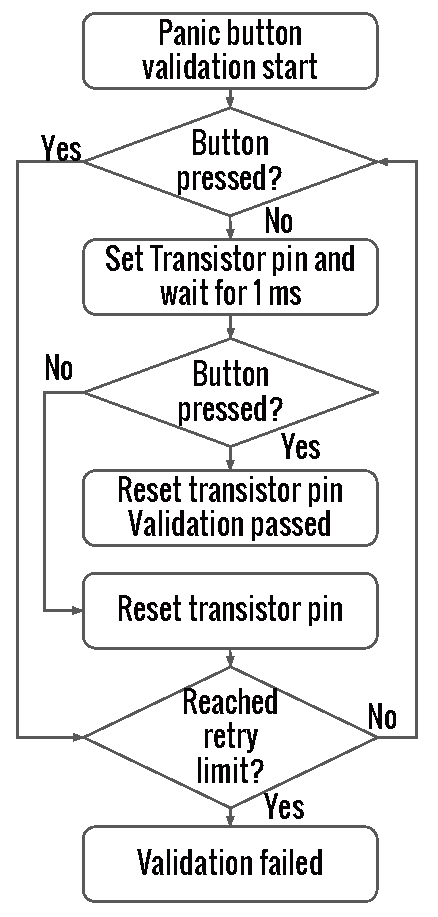
\includegraphics[scale=0.7]{panic_button_validation.pdf}
\caption{Flow chart of Panic Button Validation}
\label{fig:panic_button_validation}
\end{figure}
\subsubsection{Firmware validation}
Firmware validation is done after every soft/hard reset. To validate the firmware MD5 checksum is calculated for entire firmware and it is compared with the MD5 checksum stored in a non-volatile memory of core-module. If both match then firmware validation passes.
\subsubsection{Tamper detection}
We use an ultra low power MSP430 microcontroller for always-on tamper detection with its independent battery. Tamper is detected using a switch mounted inside the enclosure. MSP430 detects the tamper by detecting the change in logic level (from high level to low level) of this switch's pin. Once tamper is detected by MSP430 microcontroller, it permanently deletes the private key stored in the flash of the microcontroller. While servicing the device, lid opening will trigger the tamper detection event, but it can be suppressed by the server by the request of an authorized personal. The private key can be retrieved from the server and re-flashed into the flash of the microcontroller by an authorized personal.\\
The core-module regularly communicates with MSP430 and sends it a unique random number. MSP430 encrypts the number using TEA encryption algorithm (explained below) and sends it back. The core-module decrypts the number back from received data, on receiving mismatched numbers, tampering is notified to the server. The flow chart is shown in the figure~\ref{fig:tamper_proof}.
\begin{figure}[H]
\centering
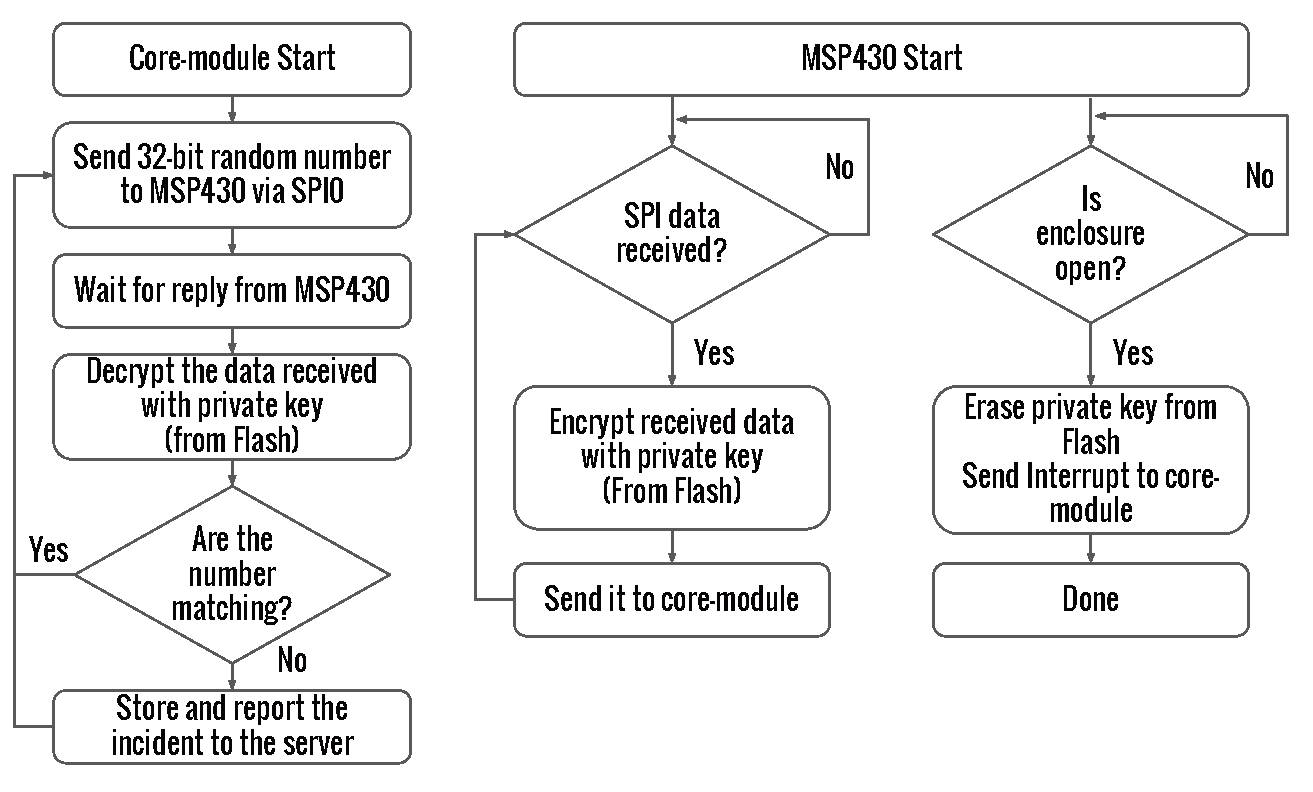
\includegraphics[scale=0.7]{tamper_proof.pdf}
\caption{Flow chart of tamper detection module}
\label{fig:tamper_proof}
\end{figure}
\paragraph{Encryption Algorithm\\}
The algorithm used is a modified version of Tiny Encryption Algorithm\cite{tea_paper}. Pseudo code of encrypt and decrypt subroutines are described in the figure~\ref{fig:msp_encryption}, where data variable is a 32-bit data to be encrypted and key is the 64-bit private key used to encrypt it.
\begin{figure}[H]
\centering
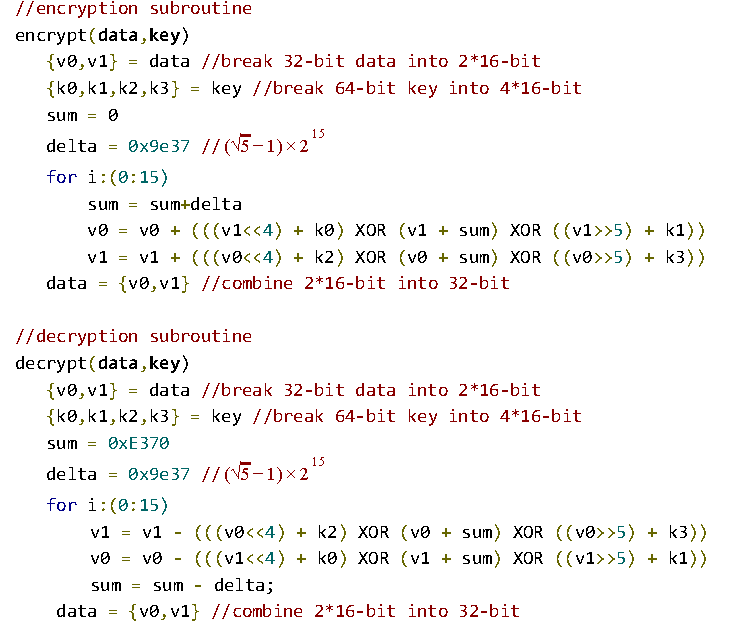
\includegraphics[width=\textwidth]{msp_encryption.pdf}
\caption{The pseudo code for the TEA encryption algorithm}
\label{fig:msp_encryption}
\end{figure}
The constants used are delta 0x9e37 ($(\sqrt{5}-1)*2^{15}$) and sum 0xE370 ((delta*16)*0xFFFF).
\subsection{Audio streaming module}
Streaming of realtime audio data with minimum latency is essential to the system for further analysis and storage as evidence in the hard-drives of the server.
Raw data is not suitable for streaming because of the sheer size of it. To compress the data, we have used Vorbis ogg\cite{vorbis_site} open-source patent free audio compression format, which is suitable the streaming and storage of audio data.\\
we used raw TCP socket to stream the audio data from the \emph{PanicButton device} to the server. We need a single stream of audio from the device, so the overhead of HTTP header is not required. The extra information required by the server is embedded inside the Vorbis ogg comments page. The data flow is shown in figure~\ref{fig:vorbis_stream}.
\begin{figure}[H]
\centering
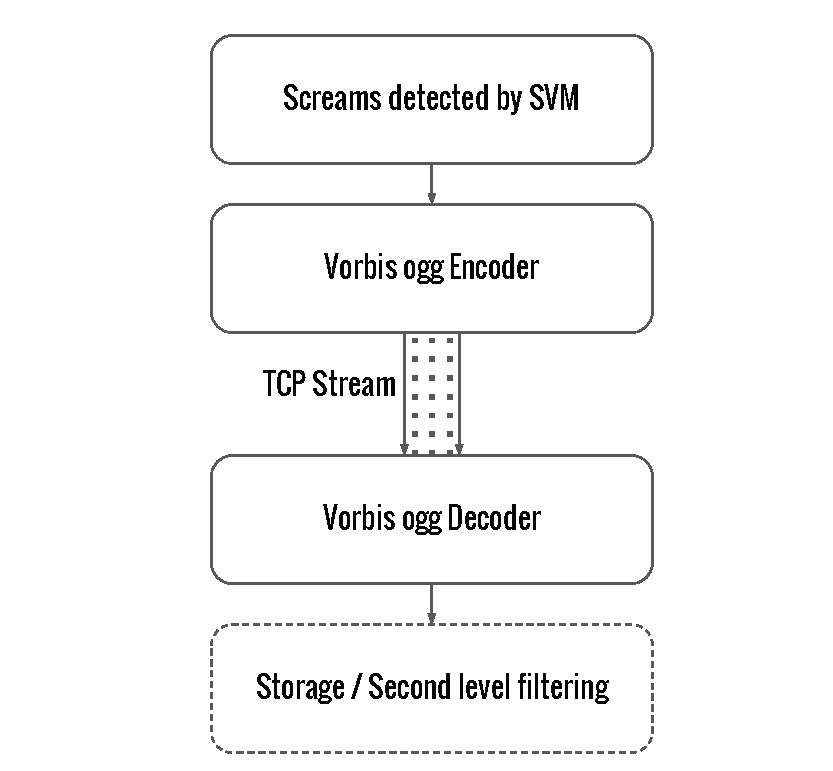
\includegraphics[scale=0.7]{vorbis_stream.pdf}
\caption{Data flow in streaming of audio data}
\label{fig:vorbis_stream}
\end{figure}
We used libvorbis, libogg and libvorbisenc open source libraries to encode and decode from the vorbis ogg format.

\subsection{Global positioning system module}
The NEO-6M module from ublox uses UART protocol for sending the GPS data to the host controller. It sends data in National Marine Electronics Association(NMEA) format. NMEA format consists of sentences, whose first word is called the data type, which defines the interpretation of the rest of the sentence. The NEO-6M module sends data with GPGGA and GPRMC data types. Core-module decodes the location and date-time information from the NMEA format.
\subsection{Panic button module}
The system needs realtime button response. To minimize the response latency, we used pin interrupt and timer combination  debouncing technique instead of using only timer based debouncing as shown in figure~\ref{fig:pin_interrupt}
\begin{figure}[H]
\centering
\includegraphics[width=\textwidth]{pin_interrupt.pdf}
\caption{Deboncing technique(a) Combination of pin interrupt and timer to reduce latency. (b) Only using timer interrupt.}
\label{fig:pin_interrupt}
\end{figure}
%TODO
The maximum period of debouncing is expected to be around 10ms\cite{debounce_paper}. We used timer tick period of 15 ms, which is greater than maximum debouncing period. In case (b) maximum latency is 15 ms and in case (a) maximum latency is of  only six cycles (0.375 us) for pin interrupt. Hence we opted for method (a).

\subsection{Audio-based trigger module}
As described in study section, we decided to use Support Vector Machine (SVM) as underlying machine learning algorithm and Mel-Frequency Cepstral Coefficients (MFCC) as feature set for this algorithm  to detect scream. Let's have a look at feature extraction procedure used in this project.
\subsubsection{Feature Extraction}
Mel-Frequency Cepstral Coefficients (MFCC), which acts as feature set, are extracted from live stream of input audio. Figure~\ref{fig:Featureextraction} depicts the Feature extraction procedure.

\begin{figure}[H]
\centering
\def\svgwidth{\textwidth}
\input{feat.pdf_tex}
\caption{Feature extraction process}
\label{fig:Featureextraction}
\end{figure}

Every second audio data is fetched from sound card and dumped into an input fifo, this 1 second of audio data is then appended with previous 0.98 second (0.98 second is multiple of 30 ms, which is the window size used in the FFT operation) of audio data. MFCC features are extracted for this composite audio clip.

MFCC are computed by first chopping the audio signal into tiny overlapping segments, these segments are multiplied with a window function like Hamming window; Fourier transform is computed over this windowed audio segment. The power spectrum is wrapped according to Mel-scale to adapt the frequency resolution of human ear. This spectrum is then segmented into number of critical bands using a triangular filter bank; Inverse Discrete Cosine Transform (DCT) applied to the logarithm of filter bank's outputs result in MFCC vector.

We obtain super feature vector of R\textsuperscript{24} for each 1.98 sec of audio data. This super feature vector is obtained by taking column mean and standard deviation of 169 x 12 matrix, which was obtained by extracting MFCC(ignoring 0\textsuperscript{th} MFC coefficient) for audio data of 1.98 sec. Once features are extracted, they are used for training the SVM.  

\subsubsection{Training of SVM}
\paragraph{Training-\\}

Like all machine learning algorithms, we need to train our SVM using a labeled data set. Labeled data set contains data that is painstakingly labeled by a human, classifying whether a particular 1.98 second clip is a scream. Clip is labeled 1 for a scream and -1 for not a scream. Figure~\ref{fig:train} depicts the training process.
 
\begin{figure}[H]
\centering
\def\svgwidth{\textwidth}
\input{train.pdf_tex}
\caption{Training process of the SVM}
\label{fig:train}
\end{figure} 
Support Vector Machine (SVM) uses a kernel to transform data into higher dimension space and finds a linear separating hyper plane with maximal margin in this higher dimensional space. We are using radial basis function (RBF) as kernel, due to its ability to model complex data patterns. RBF kernel \(K(x_i,x_j)\)
is defined as- \[K(x_i,x_j)=exp(-\gamma\parallel(x_i-x_j)\parallel^2), \gamma>0.\]
For training SVM that uses RBF kernel, we need to specify values of two parameters -
\begin{enumerate}
 \item C (penalty factor used in cost function) and 
 \item \(\gamma\) ( variance of the RBF kernel).
\end{enumerate}
 We used following steps to get optimum value of C and \(\gamma\) and use them for the training-
\begin{enumerate}
\item Arrange data in proper format i.e., [data,label],
\item Randomize the data in cross-validation set,
\item Consider the RBF kernel \(K(x,y)=e^{(-\gamma\parallel(x_i-x_j)\parallel^2)}\),
\item Use cross-validation set to find the best values for parameters C and \(\gamma\),
\item Use these values of C and \(\gamma\), to train the SVM from training data set and
\item test.
\end{enumerate}

We will dwell into details of these steps in section \ref{sssec:FindCandgamma}, first lets have a look at data set used in this project. 

\paragraph{Data set-\\}

Data set used in this project is called IIITD Urban Environment Context database (IUEC)\cite{paper10}. It contains audio clips from following environmental contexts-
\begin{enumerate}
\item Conversation (narrations)
\item Human gathering (clubs and meetings)
\item Indoors (indoor sounds)
\item machinery (fan, shaver, laptop-fan, exhaust, oven, mixer, washing machine and vacuum cleaner)
\item Multimedia (movie audio and TV audio)
\item Outdoors (bus stand, road traffic, market, temple, rickshaw, rain, metro and playground)
\item distress (scream and crying sounds)
\end{enumerate}

Table~\ref{tab:quandata} quantifies the content of this dataset.
\begin{table}[H]
\begin{center}
\begin{tabular}{ |c|c| } 
 \hline
 \textbf{Context} & \textbf{Samples of 2 sec} \\ 
 \hline
 \hline
 Conversation & 623 \\
 \hline 
 Human gathering & 1621 \\ 
 \hline
 Indoors & 4169 \\
 \hline
 Machinery & 3548 \\
 \hline
 Multimedia & 3698 \\
 \hline
 Outdoors & 5142 \\
 \hline
 Scream & 464 \\
 \hline
 \hline
 \textbf{Total} & \textbf{19265= 10 Hrs 42 Mins}\\
 \hline
\end{tabular}
\end{center}
\caption{IUEC Data set details} \label{tab:quandata}
\end{table}

Apart from this data set, we collected data using the \emph{PanicButton device} prototype. Table~\ref{tab:quandata2} quantifies its content.
\begin{table}[H]
\begin{center}
\begin{tabular}{ |c|c| } 
 \hline
 \textbf{Context} & \textbf{Samples of 2 sec} \\ 
 \hline
 \hline
 Conversation & 1144 \\ 
 \hline
 Multimedia & 1828 \\
 \hline
 Outdoors & 2623 \\
 \hline
 Scream & 464 \\
 \hline
 \hline
 \textbf{Total} & \textbf{6059= 3 Hrs 22 Mins}\\
 \hline
\end{tabular}
\end{center}
\caption{Details of data collected from panic button prototype} \label{tab:quandata2}
\end{table}

Scream samples were obtained by re-recording scream data available in IUEC data set. We combined this two data sets to get a composite data set, whose content is quantified in Table~\ref{tab:quandata3}
\begin{table}[H]
\begin{center}
\begin{tabular}{ |c|c| } 
 \hline
 \textbf{Context} & \textbf{Samples of 2 sec} \\ 
 \hline
 \hline
 Conversation & 1767 \\
 \hline 
 Human gathering & 1621 \\ 
 \hline
 Indoors & 4169 \\
 \hline
 Machinery & 3548 \\
 \hline
 Multimedia & 5526 \\
 \hline
 Outdoors & 7765 \\
 \hline
 Scream & 928 (3.6\% of complete data set)\\
 \hline
 \hline
 \textbf{Total} & \textbf{25324= 14 Hrs 4 Mins}\\
 \hline
\end{tabular}
\end{center}
\caption{Composite Data set details} \label{tab:quandata3}
\end{table}

This complete data set gets divided into two equal parts called training data set and cross-validation data set. Training data set is used for training the SVM and cross-validation dataset is used for tuning the SVM. Our data set is highly skewed i.e., scream samples constitutes only 3.6\% of the complete data set. This makes benchmarking of trained SVMs non-conventional. Section~\ref{sssec:FindCandgamma} addresses this problem in detail.

Finally, a test clip of 22 minutes was created to quantify performance of the trained SVM. This 22 minute clip was carefully designed to cover audio samples from every context. Obtained results are mentioned in Section~\ref{sssec:performanceSVM}.

\subsubsection{Finding C and gamma} 
\label{sssec:FindCandgamma}
To find the optimum value of C and \(\gamma\), we performed grid search for these parameters on cross-validation data set. Five fold cross-validation data set (4 part for training and 1 part for testing in circular fashion for a particular combination of C and \(\gamma\)) is used. Figure~\ref{fig:CVflowchart} shows the process of finding optimum C and \(\gamma\).

\begin{figure}[H]
\centering
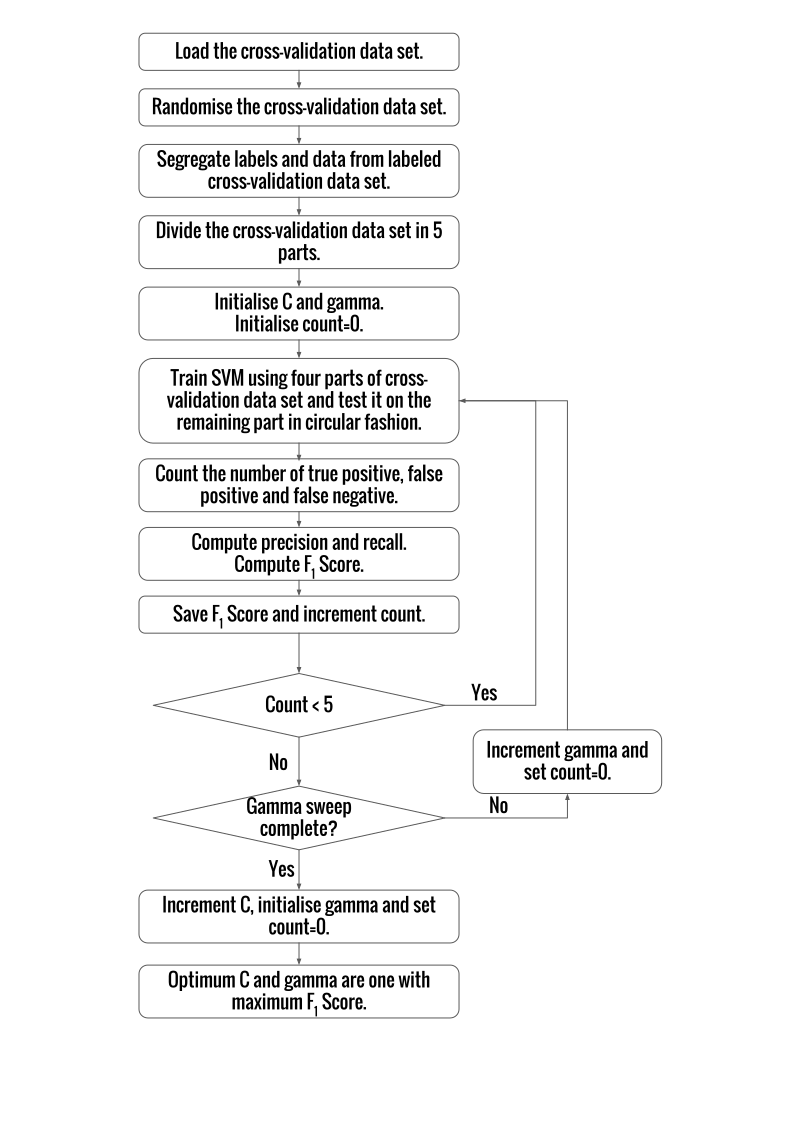
\includegraphics[scale=0.85]{CVflowchart.pdf}
\caption{Cross-validation process for obtaining optimum C and gamma}
\label{fig:CVflowchart}
\end{figure}

Method shown in figure~\ref{fig:CVflowchart} is a brute force method to find optimum value of C and \(\gamma\). We use \(F_1\) score as figure of merit (FOM); Accuracy can't be used as FOM due to skewed nature of data set.

\(F_1\) score is computed using precision (prec) and recall (rec):\[F_1=\dfrac{2 . prec . rec}{prec+rec},\] We can compute precision and recall by: \[prec=\dfrac{t_p}{t_p+f_p}\]
\[rec=\dfrac{t_p}{t_p+f_n}\]
where
\begin{itemize}
\item \(t_p\) is the number of true positives: the ground truth label says it's a scream and our algorithm correctly classified it as a scream.
\item \(f_p\) is the number of false positives: the ground truth label says it's \textbf{not} a scream, but our algorithm incorrectly classified it as a scream.
\item \(f_n\) is the number of false negatives: the ground truth label says it's a scream, but our algorithm incorrectly classified it as \textbf{not} a scream.
\end{itemize}

In any automated alarm system, ideally we should have zero false negative, practically it should be as small as possible. Following figure show us the $F_1$ score obtained by performing grid search for the parameters C and \(\gamma\) on the cross-validation set.
\begin{figure}[H]
\centering
\def\svgwidth{\textwidth}
\input{F1score.pdf_tex}
\caption{F1 score obtained from grid search for C and gamma on CV set}
\label{fig:f1score}
\end{figure} 

Once we have the value of C and \(\gamma\), we can use that value to train our SVM. This process of first obtaining appropriate value of C and \(\gamma\) and then training the final SVM, helps us in avoiding machine learning traps like over-fitting and under-fitting.
Performance of the trained SVM is quantified in section~\ref{sssec:performanceSVM}, besides figure~\ref{fig:f1score} also quantifies the performance of best SVM, over the five fold cross-validation set.

\subsubsection{Performance of the SVM}
\label{sssec:performanceSVM}

We performed benchmarking using a 22 minute test set, this test set contains 24 screams of different lengths and strengths. We were able to detect 23 screams with 1 false negative and 3 false positive, giving us accuracy of \textbf{95.8\%} and \(F_1\) score of \textbf{0.92} with latency of 1.480 ms.


%Based on the input and output stimuli classification of each %software
%module or sub-module, perform the algorithm design which includes,
%\begin{itemize}
%\item numeric format for the application in case of embedded %software (floating
%point or fixed point and positioning of the virtual binary point)
%\item normalising and scaling constants
%\item module inputs and type
%\item module output and type
%\item module constants
%\item global constants
%\item referred subroutines
%\item algorithm in pseudocode
%\end{itemize}
%NOTE: \emph{include as many sections/sub-sections as there are %software
%modules/sub-modules and repeat the above for every software module
%and sub-module}.


\section{Industrial design}
\subsection{Module design}
Connected panic button's industrial design is divided as follows-
\begin{itemize}
\item Design of top panel,
\item Design of panic button,
\item Design for the tamper detection circuit and,
\item Design of the base.
\end{itemize}

\subsubsection{Design of top panel}
Top panel of the \emph{PanicButton device} acts as host to emergency button, speaker and microphone. The panic button's stem passes through the center of the front panel. Just beside the grove for passing the stem of emergency button, is a whole of radius 4 cm, which acts as speaker housing. One more hole of radius 0.5 cm is kept besides the house of speaker for mounting microphone. 

Speaker and microphone are assembled in a manner that the sound produced from speaker gets directly coupled to the microphone from outside the enclosure. A cap was designed around the speaker, to minimize the coupling of sound from inside the enclosure. Bottom part of the panic button plays an important role in this coupling of audio and is discussed in section~\ref{sssec:designemergency}. Figure~\ref{fig:toptop} shows the top view of the top panel and figure~\ref{fig:bottomtop} shows the bottom view of the top panel.

\begin{figure}[H]
\centering
\includegraphics[width=\textwidth]{untitled_231.jpg}
\caption{Top view of the top panel of the \emph{PanicButton device}}
\label{fig:toptop}
\end{figure}

\begin{figure}[H]
\centering
\includegraphics[width=\textwidth]{untitled_241.jpg}
\caption{Bottom view of the top panel of the \emph{PanicButton device}}
\label{fig:bottomtop}
\end{figure}

\subsubsection{Design of panic button}
\label{sssec:designemergency}
To make panic button easily accessible at all times, we took care of following two things.
\begin{itemize}
\item Area of the panic button equals the average area of a adult human's palm and
\item Back-light is added to the panic button to make sure that it is easily visible in the night. 
\end{itemize}

An important part of the emergency button design is to make sure that the button does not cover the microphone, while completely covering the speaker; Proper placement of these three component and size of button can take care of this.

Bottom part of the panic button acts as a reflector for sound produced by the speaker. For efficient performance of microphone validation procedure, it is important that the waves produced by the speaker are channeled to the microphone. To accomplish this task, bottom part of panic button was given a concave shape such that microphone lies at the focal point of the concave surface.

Stem of the emergency button was made hollow to pass wires for the back-light mounted inside the emergency button.
 
\subsubsection{Design for the tamper detection circuit}
Tamper detection circuit takes the input from a push button, that gets pushed once the top panel is mounted on the base of the enclosure. We designed a projection coming out of the wall to support the mounting of the switch. Figure~\ref{fig:tamper_detection_switch} shows the placement and shape of the projection.

\begin{figure}[H]
\centering
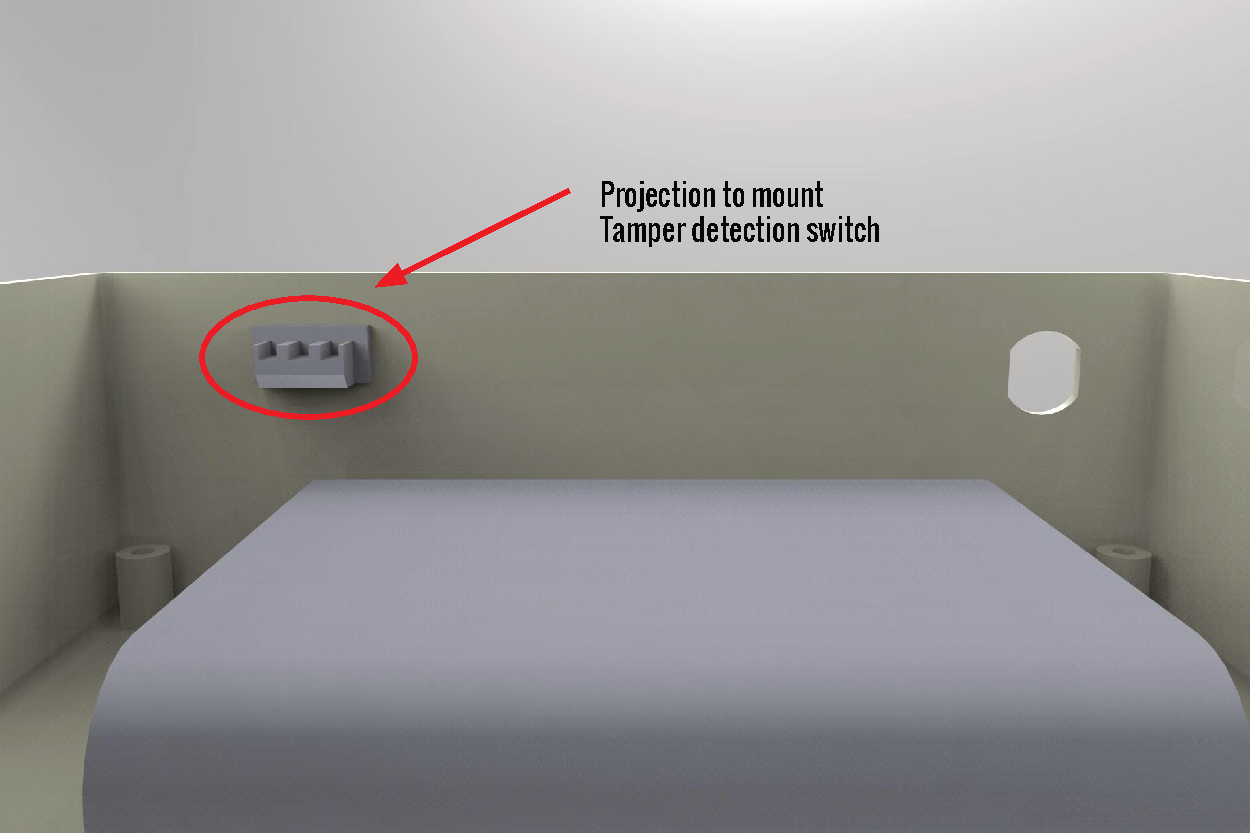
\includegraphics[width=\textwidth]{tamper_detection_switch}
\caption{The projection to mount the tamper detection switch}
\label{fig:tamper_detection_switch}
\end{figure}  

\subsubsection{Design of the base}
The base of the enclosure act as the host for all components residing inside the \emph{PanicButton device}. We placed 4 mounting holes for the raspberry pi and 4 m3 screw holes for bringing top and base together.

\subsection{Putting modules together}
\label{sec:desIndust}
Figure~\ref{fig:des_views} shows the \emph{PanicButton device}, once all modules are brought together and figure~\ref{fig:exploded_views} shows the exploded view of the \emph{PanicButton device}.  
\begin{figure}[H]
\begin{subfigure}{.5\textwidth}
  \centering
  \includegraphics[width=.9\linewidth]{des_top_view}
  \caption{Top view}
  \label{fig:des_top_view}
\end{subfigure}%
\begin{subfigure}{.5\textwidth}
  \centering
  \includegraphics[width=.9\linewidth]{des_side_view}
  \caption{Side view}
  \label{fig:des_side_view}
\end{subfigure}
\begin{subfigure}{.5\textwidth}
  \centering
  \includegraphics[width=.9\linewidth]{des_front_view}
  \caption{Front view}
  \label{fig:des_side_view2}
\end{subfigure}%
\begin{subfigure}{.5\textwidth}
  \centering
  \includegraphics[width=.9\linewidth]{des_iso_view}
  \caption{Isometric view}
  \label{fig:des_iso_view}
\end{subfigure}
\caption{Top, side, front and isometric views of the enclosure}
\label{fig:des_views}
\end{figure}

\begin{figure}[H]
  \centering
  \includegraphics[width=.8\linewidth]{exploded_iso}
\caption{Exploded views of the enclosure}
\label{fig:exploded_views}
\end{figure}

%The section should include the following
%\begin{itemize}
%\item enclosure design (considering function, ergonomics and aesthetic)
%\item front panel design
%\item back panel design
%\item inter-module wiring and interconnection routing
%\item issues and considerations related to user interactions
%\item issues related to maintainability
%\item exploded view\end{itemize}



\chapter{Engineering and fabrication} 

%This chapter includes all the engineering and fabrication details
%needed to develop the product. 

\section{Product structure}
The product looks like a simple box from outside but it's more than that. Beneath the button is a speaker and beside it lies a microphone. Top panel is a 3D printed panel, housing emergency button, speaker and microphone. Bottom side of top panel takes care of connection between the custom build button assembly and a push button switch, provides support for speaker housing and a projection to press push button of tamper detection module. The base hosts most of the electronics. Half of the base part is occupied by raspberry pi and its add-on board, other half is occupied by the battery and its charging circuitry. Side wall of base part exposes power connector to charge the secondary battery and power the entire electronics. Figure~\ref{fig:block_dia} shows the block diagram of the complete design.\\
In this chapter, we look at hardware tools, software tools and assembly/fabrication procedures required to make \emph{PanicButton device}. 

\begin{figure}[H]
\centering
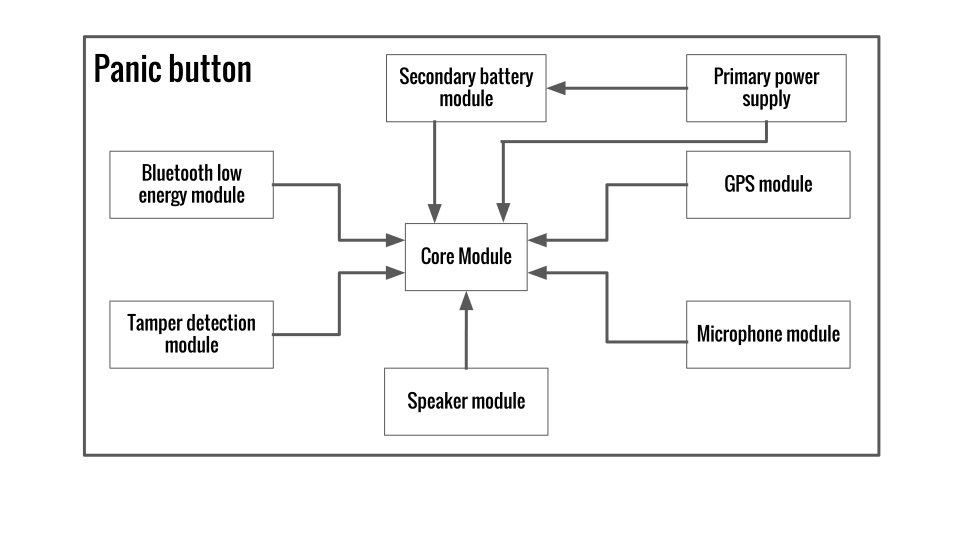
\includegraphics[width=\textwidth]{block_dia}
\caption{Block diagram of the \emph{PanicButton device}}
\label{fig:block_dia}
\end{figure}

%This section provides the overall structure of the product in a top-down
%manner as viewed by a person when opening up the product completely
%to its component parts. The overall structure is given with the help
%of a block diagram schematic. On some modules, embedded software may
%reside and its structure diagram can be shown separately module-wise.
%The structure diagram for any standalone software should also be included.


\section{Hardware modules}
The \emph{PanicButton device} can be divided into three parts namely raspberry pi, add-on board for raspberry pi and the enclosure. Base part of the enclosure acts the hosing for these modules.

\subsection{Raspberry pi}
Raspberry pi's sd card with modified Raspbian image, must be installed into the raspberry. Raspberry pi should be mounted on the base using four M2 screws of 0.5 cm length.

\subsection{Add-on board for raspberry pi}
Add-on board contains the BLE module, programming header for BLE module, GPS module, speaker module, emergency button headers and tamper detection module. Figure~\ref{fig:schematic} shows the circuit schematic for the raspberry pi's add-on board.

\begin{figure}
\centering
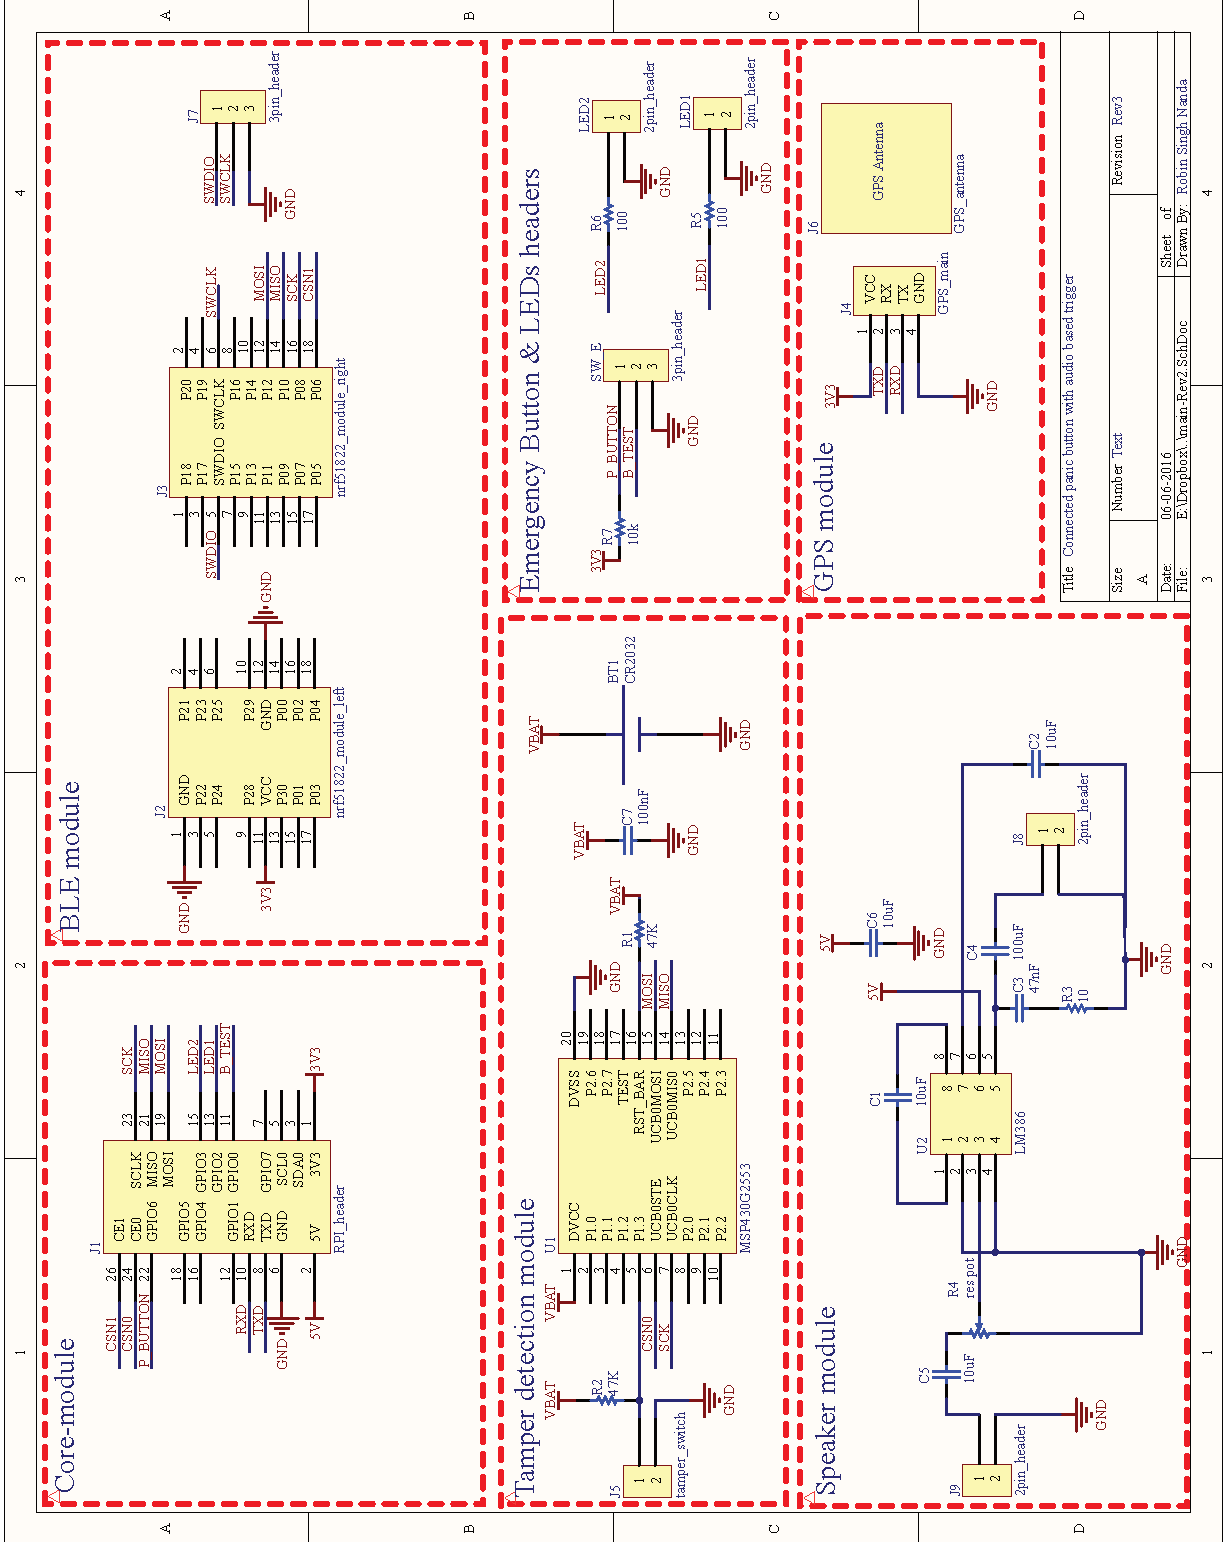
\includegraphics[width=\textwidth]{schematic}
\caption{Schematic of raspberry Pi add-on board}
\label{fig:schematic}
\end{figure}
The add-on board has a non rectangular shape because of the ethernet and USB connectors of the raspberry pi. Mounting holes of the add-on board are aligned to the mounting holes of the raspberry pi board. Figure.~\ref{fig:enc_top_view} shows the top layer of add-on board's PCB and figure.~\ref{fig:enc_bottom_view} shows the bottom layer of the add-on board's PCB. Our application did not impose any constrain on the thickness of the substrate, hence common substrate of 1.6 mm thickness was used. All signal tracks on the PCB are of 10 mil width. The add-on board connects to raspberry pi via 26 pin female header and can be secured using M3 mounting screws.

\begin{figure}[H]
\begin{subfigure}{.5\textwidth}
  \centering
  \includegraphics[width=.95\linewidth]{pcb_top}
  \caption{Top side}
  \label{fig:enc_top_view}
\end{subfigure}%
\begin{subfigure}{.5\textwidth}
  \centering
  \includegraphics[width=.95\linewidth]{pcb_bottom}
  \caption{Bottom side}
  \label{fig:enc_bottom_view}
\end{subfigure}
\caption{Top side and bottom side of PCB of Raspberry pi add-on board}
\label{fig:enc_views}
\end{figure}

Figure~\ref{fig:bom} shows the bill of materials used in this project.
\begin{figure}
\centering
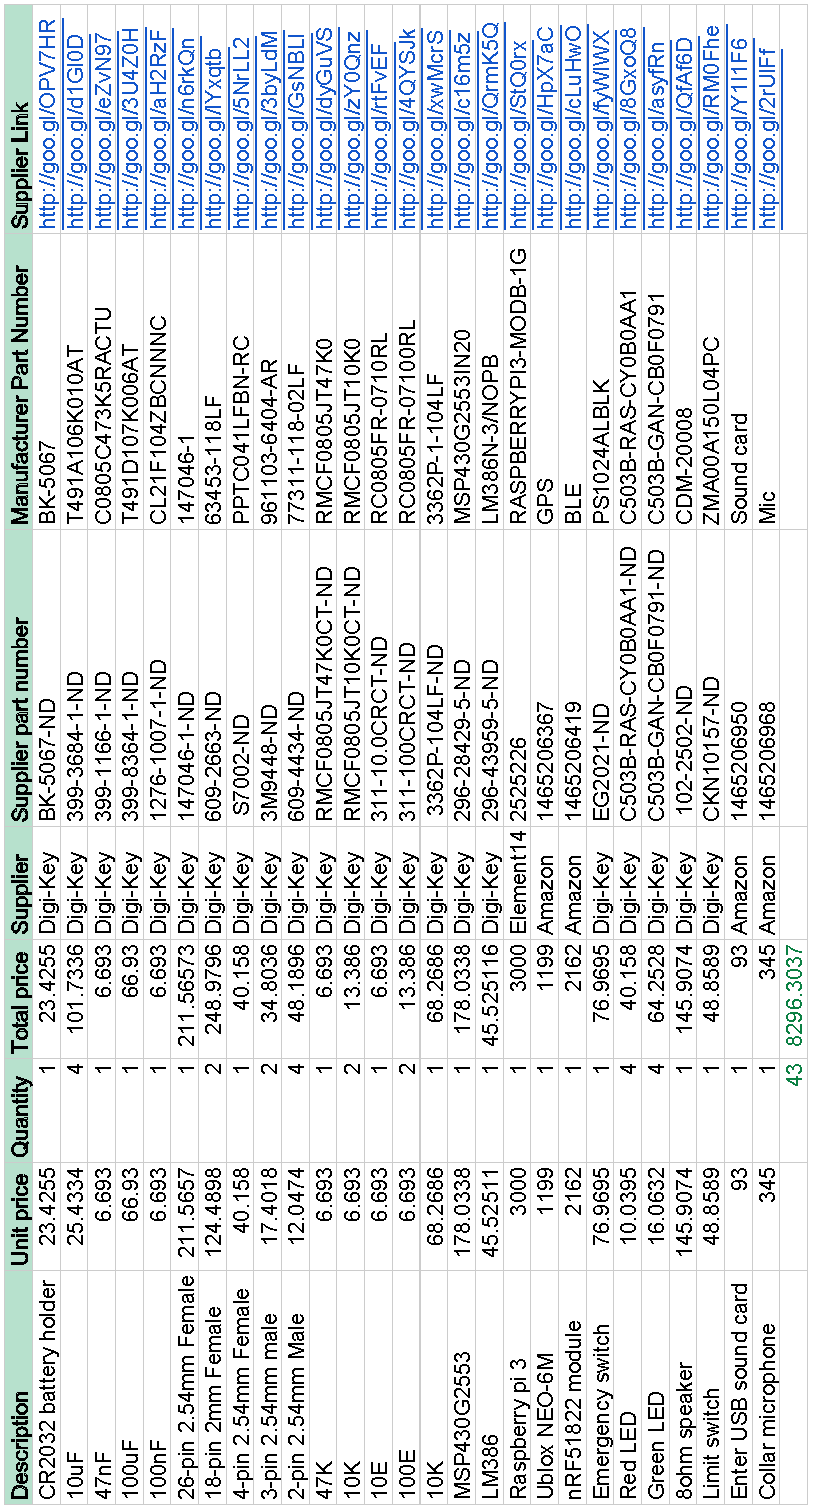
\includegraphics[width=0.8\textwidth]{bom}
\caption{Bill of materials}
\label{fig:bom}
\end{figure}
\subsection{Enclosure of \emph{PanicButton device}}
Enclosure was fabricated using a 3D printer that uses fused deposition modeling technique. Many parts of top panel were fabricated individually. Figure ~\ref{fig:enc_views} shows different views of the fabricated panic button enclosure. 

\begin{figure}
\begin{subfigure}{.5\textwidth}
  \centering
  \includegraphics[width=.9\linewidth]{enc_top_view}
  \caption{Top view}
  \label{fig:enc_top_view}
\end{subfigure}%
\begin{subfigure}{.5\textwidth}
  \centering
  \includegraphics[width=.9\linewidth]{enc_side_view}
  \caption{Side view}
  \label{fig:enc_side_view}
\end{subfigure}
\begin{subfigure}{.5\textwidth}
  \centering
  \includegraphics[width=.9\linewidth]{enc_side_view2}
  \caption{Front view}
  \label{fig:enc_side_view2}
\end{subfigure}%
\begin{subfigure}{.5\textwidth}
  \centering
  \includegraphics[width=.9\linewidth]{enc_iso_view}
  \caption{Isometric view}
  \label{fig:enc_iso_view}
\end{subfigure}
\caption{Different views of the enclosure}
\label{fig:enc_views}
\end{figure}

%For every hardware module, the following engineering and fabrication
%details should be included,
%\begin{itemize}
%\item physical dimensions with mounting hole details
%\item connectors and connector pin details with pin-level labeling
%\item circuit diagram using connector pin-level labeling as inputs and outputs
%\item printed circuit board layout with circuit and connectors
%\item routing details
%\item drilling details
%\item assembly and mounting details
%\item bill of materials with cost
%\item vendor details
%\item development setup details: schematic editor, layout editor etc. ,
%assembly requirements, software for writing embedded software if any,
%debugging tools, JTAG tools, power supply requirements, monitoring
%requirements like CRO and multimeters etc.
%\item Testing procedure for validating the module
%\end{itemize}
%NOTE: include sections for every hardware molude and include the details
%as indicated above.


\section{Software modules}
\subsection{Raspberry pi core-firmware}
All the firmware of raspberry pi core is implemented in java language, which requires Oracle JavaSE v8 to run, can be installed using the following command.\\
\emph{sudo apt-get install oracle-java8-jre}\\
The firmware for raspberry pi is developed using Intellj Idea Ultimate 2016.1 Integrated Development Environment (IDE). The firmware is packaged in Java archive (JAR) file. The raspberry pi must run the jar file on boot up.
\subsection{nRF51822 firmware}
The firmware for nRF51822 based Bluetooth low energy module is developed using Keil $\mu$Vision 5 IDE. The firmware is written in plain C and packaged into a hex file, which can be programmed to nRF51822 SOC using Serial Wire Debug (SWD) interface using Segger Jlink debugger.
\subsection{MSP430 firmware}
The firmware for MSP430 module is developed using Texas Instruments Code Composer Studio (TI-CCS). The firmware is written in plain C and packaged into a hex file, which can be programmed to MSP430 microcontroller using Texas Instruments MSP-FET430UIF debugger or Texas Instruments MSP430 Launchpad debugger.
\subsection{Scream detection firmware}
Scram detection algorithm was implemented in GNU Octave 3.8.2. Octave is a high-level interpreted language, primarily intended for numerical computations. It provides capabilities for the numerical solution of linear and nonlinear problems, and for performing other numerical experiments. GNU Octave can be installed in linux machine using following command-\\
\emph{sudo apt-get install octave}\\
Signal and image package of octave are also required for machine learning firmware development. These packages can be install using following commands.\\
\emph{sudo apt-get install octave-signal}\\
\emph{sudo apt-get install octave-image}
\subsection{Server code}
The server code is tested for running on Mosquitto MQTT borker v1.4.8, Apache tomcat server v8 and MySQL database  server v5.7.12, other versions of servers might not work as expected. The server code is developed in Intellj Idea Ultimate 2016.1.  The server code can be divided into the following parts.
\begin{itemize}
\item Mosquitto application code
\item Apache tomcat servlet code
\end{itemize}
\subsubsection{Mosquitto application code}
The mosquitto application code is packaged into a JAR file, which requires Oracle JavaSE v8 or higher. The mosquitto application requires Mosquitto MQTT broker and MySQL database to be running.
\subsubsection{Apache tomcat servlet code}
The apache tomcat servlet code in packed into a Web-application archive (WAR) file, which also requires Oracle JavaSE v8 or higher. The apache tomcat servlet code requires Apache tomcat server and MySQL database server to be running.

\subsection{Android app}
The Android application requires Android version 4.3 or higher and bluetooth v4.0  or higher to run reliably. The android application was developed using Android Studio v2.0. The app is packaged into a Android application package (APK) file, which can be side-loaded into the Android phone or tablet.
%For every software module, include the following,
%\begin{itemize}
%\item development setup details: debugger, tools, interconnection to PC,
%power supply etc.
%\item pseudocode of algorithm
%\item subroutine or function code listing (include line by line comments
%in code for easy comprehension of the code)
%\item compilation details: make file etc.
%\item software embedding details if any
%\item testing procedure for validating the module
%\end{itemize}


\section{Key configuration parameters}
The key configuration parameters a
\begin{table}[H]
\begin{center}
\begin{tabular}{ |c|c|c|c| } 
 \hline
 \textbf{Parameter name} & \textbf{size} & \textbf{module} & \textbf{value} \\
 \hline 
 \hline
  \emph{panicButtonID} & 128-bit & core-module & From server\\
 \hline
 \emph{publicRSAKey} & 256-bit & core-module & From server\\
 \hline
 \emph{teaKey} & 64-bit & core-module & From server\\
 \hline
 \emph{teaKey} & 64-bit & tamper-detection module & From server\\
 \hline
\end{tabular}
\end{center}
\caption{Feature extraction time using MFCC and spectral feature as feature vector} \label{tab:scr2}
\end{table}
\section{System integration}
In the following sections, we look at internal and external connections going into \emph{PanicButton device}.
\subsection{Internal connections}
\begin{itemize}
\item The raspberry pi add-on board connects to raspberry pi  using 26-pin female header which is paired to 40-pin male header.
\item The USB sound card should be connected to a USB port of the raspberry pi.
\item The audio output from raspberry pi connects to the header J9  on the add-on board.
\item The speaker connects to J8 header of add-on board.
\item The microphone connects to the mic port on the USB sound card.
\item The panic button connects to 3-pin SW\_E header on add-on board.
\item The red and green LEDs connects to LED1 and LED2 header on the add-on board respectively.
\item The GPS module connects 4-pin header J4 on the add-on board.
\item The nRF51822 BLE module connects to header J2 and J3 on the add-on board.
\item The tamper detection button connects to J5 header on add-on board.
\item The USB power from USB power bank connects to Raspberry pi power in port.
\item The USB power from USB charger connects to Power bank's power in.
\end{itemize}
\subsection{External connections}
The \emph{PanicButton device} requires a 12V DC voltage from vehicle battery or any other source, going into dc-power jack on the right side of the enclosure.
%This section should include 
%\begin{itemize}
%\item inter module hardware interconnection details
%\item inter module software interconnections
%\item interconnections between the system and external environment like
%inputs and outputs (sources and sinks)
%\item system level testing procedure for validating the system experimentally
%\item figures obtained from CRO and/or other instruments
%\item demonstration setup and the procedures for validating the system with
%target specifications\end{itemize}




\chapter{Concluding remarks}

%This chapter should include the following sections,


\section{User instructions}
\subsection{Auto validation}
User should give the Android app all the necessary runtime permissions. The smartphone internet data and BLE should be turned on. The app will automatically detect nearby panic button system and notify user once, the validation procedure completes and the details of vehicle and driver are available. If the validation fails the phone will warn user about the situation.
\subsection{Manual validation}
In case of manual validation, user should go to app on his android smartphone and tap on Validate button. This will start the validation procedure with the nearest gateway device and once the validation completes, the user will be notified with the status of validation and the details of the vehicle and driver.
\subsection{Emergency request}
The user can either press the panic button on the \emph{PanicButton device} or scream. In either case the emergency request will be sent to the nearby PCR.
%The section contains a brief user manual.


%\section{Corrections}

%This section document any last minute corrections that would have
%been undocumented in the engineering and fabrication chapter.


\section{Suggestions for next gen}
In the next gen of this device, following things can be modified-
\begin{itemize}
\item Form factor of the device, it can be made smaller.
\item Performance of the scream detection unit can be improved, through application specific training of the SVMs.
\item Porting the audio detection algorithm to a low-power microcontroller.
\end{itemize}
%This section will give your pointers, tips and recommendations for
%the next generation product and will be of great help to the future
%batch of students working on similar products.


\section{Future scope}
This product has a great potential at reducing the number of crime in public transport vehicle. That being said, the current status of product is incapable of fulfilling this vision due to its large form factor and few field trials. 
%This section will give your view point on the product and its possible
%impact in the market with a discussion on the future scope for this
%product.


%\appendix
%
\chapter{Data}

This appendix should include
\begin{itemize}
\item data related to significant system parameters
\item significant portions of data sheet
\item significant portions of standards and protocols
\item scientific data related to the product or product-system\end{itemize}


\chapter{Program Listing}

If the programs are lengthy with many functions and subroutines, then
include all the program listing in this appendix rather than in the
various modules of the engineering and fabrication chapter.

%
\chapter{Contributions}

In the process of completing the project, there may have been many
contributions towards the product. This appendix should give a list
of your contributions that have a novelty in it. These may be
\begin{itemize}
\item Ideas that can be possible intellectual property
\item Possible patentability of any of the modules
\item Conference or Journal publications\end{itemize}


\bibliographystyle{unsrt}\bibliographystyle{unsrt}
\bibliography{report}

\end{document}
